\documentclass[letterpaper,11pt]{report}

\usepackage{fullpage}
\usepackage{verbatim}
\usepackage{cite}
\usepackage{setspace}
\usepackage{fancyhdr}
\usepackage{amsmath}
\usepackage{amssymb}
\usepackage{float}
%\usepackage{noReferences}
\usepackage[small]{caption}
\usepackage{graphics}
\usepackage{color}
\usepackage{epstopdf}
\usepackage[ruled,vlined]{algorithm2e}
\usepackage[none]{hyphenat}
\usepackage{amsthm}
\theoremstyle{definition}
\newtheorem{definition}{Definition}[section]

\usepackage[bookmarks=true,%
bookmarksnumbered=true,%
colorlinks=true,%
linkcolor=linkcol,%
citecolor=citecol,%
urlcolor=urlcol,%
hypertexnames=true,%
pdfpagelabels,
]{hyperref}

\definecolor{linkcol}{rgb}{0,0,1}
\definecolor{citecol}{rgb}{0,0.5,0}
\definecolor{urlcol}{rgb}{0.3,0,0}


\hyphenpenalty 10000
\exhyphenpenalty 10000
\sloppy

\usepackage{hyperref}
%\usepackage{natbib}
\usepackage{listings}
\usepackage{color}
\usepackage{xcolor}
\usepackage[]{datetime}
%\usepackage{lipsum}
\usepackage{graphicx}
\usepackage{subcaption}

\newcommand{\code}[1]{\texttt{\scriptsize{#1}}}
\newcommand{\mycomment}[1]{}
\newcommand{\todo}[1]{\textbf{TODO: #1}}
\newcommand{\mytab}{~~~~}
\newcommand{\sspace}{~}
\newcommand{\etal}{\textit{et al.}}
\newcommand{\eg}{{e.g.,}}
\newcommand{\ie}{{i.e.,}}
\newcommand{\lno}[1]{{\tiny{\textbf{(#1)~~}}}}

\def\tool{\textsc{Clotho}\xspace}

\newcommand{\java}{\textsc{Java}}
\newcommand{\soot}{\textsc{Soot}}
\newcommand{\infoflow}{\textsc{InfoFlow}}
\newcommand{\sdn}{{SDN}}
\newcommand{\verifier}{\textsc{Verifier}}
\newcommand{\validator}{\textsc{Flow\_Consistency\_ Validator}}
\newcommand{\outputs}{{\mathbb O}}
\newcommand{\stream}{{\mathbb S}}


\definecolor{dkgreen}{rgb}{0,0.6,0}
\definecolor{gray}{rgb}{0.5,0.5,0.5}
\definecolor{mauve}{rgb}{0.58,0,0.82}

\lstset{frame=tb,
  language=Java,
  aboveskip=3mm,
  belowskip=3mm,
  showstringspaces=false,
  columns=flexible,
  basicstyle={\small\ttfamily},
  numbers= left,
	numbersep=6pt,
	numberstyle=\small,
  %frame=single,
  numberstyle=\tiny\color{gray},
  keywordstyle=\color{blue},
  commentstyle=\color{dkgreen},
  stringstyle=\color{mauve},
  breaklines=true,
  breakatwhitespace=true
  tabsize=2
	morecomment=[l]{//} 
	escapeinside={<@}{@>}
}
 % define the title
 
% Paper conservation layout. Long live the trees!!
\setlength{\oddsidemargin}{-0.4mm} % 25 mm left margin
\setlength{\evensidemargin}{\oddsidemargin}
\setlength{\textwidth}{160mm}      % 25 mm right margin
\setlength{\topmargin}{-5.4mm}     % 20 mm top margin
\setlength{\headheight}{5mm}
\setlength{\headsep}{5mm}
\setlength{\footskip}{10mm}
\setlength{\textheight}{225mm}     % 20 mm bottom margin

\setlength{\parskip}{1ex}
\parindent 0in

% \def\SAONE{Specific Aim 1}
% \def\SATWO{Specific Aim 2}
% \def\SATHREE{Specific Aim 3}
% \def\SAFOUR{Specific Aim 4}

\renewcommand\lstlistingname{Code Snippets}
\renewcommand\lstlistlistingname{List of Code Snippets}


\def\title{Mytitle}
%\def\titletwo{Thesis Proposal Title Line 2}
\begin{document}



\def\addrone{IIIT-Delhi, Okhla Phase 3}
\def\addrtwo{New Delhi, India}

\begin{center}
%\textcolor{red}{\textbf{Draft Version \today}}
\end{center}


\def\degree{M.Tech. in Computer Science with Specialization in Information Security}


\def\submissiondate{December 08, 2014}

\def\supervisorone{Dr. Rahul Purandare}
\def\external{Dr. Mohan Dhawan}
\def\internal{Dr. Sambuddho Chakravarty}

%\def\supervisortwo{Shishir Nagaraja}
%
%
%\def\supervisorthree{Gaurav Gupta}
%
%
%\def\supervisorfour{XXX XXXX }
%
%
%\def\supervisorfive{YYY YYYY}

\thispagestyle{empty}

\begin{center}

{\LARGE \bf {\tool: Saving Programs from Malformed Strings and Incorrect
String-handling}

 }  
 \vspace{.3in}
 
 {\Large{Student Name: Aritra Dhar}} \\  
 \vspace{.1in} 
 IIIT-D-MTech-CS-IS-12-004 \\

 Nov 25, 2014 \\
  
    \vspace{.35in}

  \vspace{.25in}

{Indraprastha Institute of Information Technology\\
New Delhi}

\vspace{.35in}  {\underline{Thesis Committee}} \\ 
\supervisorone~(Advisor) \\
\external~(External reviewer) \\
\internal~(Internal reviewer)
% \\ \supervisortwo \\ \supervisorthree \\ \supervisorfour \\  \supervisorfive}
  \\ \vspace{.35in}


 {Submitted in partial fulfillment of the requirements \\for the Degree of M.Tech. in Computer Science, \\ with specialization in Information Security}

\vspace{1.2in}


\copyright 2014 Aritra Dhar \\ All rights reserved \\
\vspace{.8in}


\end{center}

%This research was partially funded by XXXX YYYY.



\newpage

\pagestyle{empty}
\vspace*{7.1in} 
\textbf{Keywords}: Software Engineering, Program Repairing, Availability,
Program Analysis, Static Analysis, Exception

\newpage

%\doublespacing
\onehalfspacing
%%%%%%%%%%%%%%%%%%%%%%%%%%%%%%%%%%%%%%%%%%%%%%%%%
%Certificate

\begin{center}
\section*{Certificate}
\label{section:certificate}
\end{center}

This is to certify that the thesis titled \textbf{``Program Repairing using
Exception Types, Constraint Automata and Typestatee"} submitted by
\textbf{Aritra Dhar} for the partial fulfillment of the requirements for the
degree of \emph{Master of Technology} in \emph{Computer Science \& Engineering}
is a record of the bona fide work carried out by him under my guidance and
supervision in the Program Analysis Research group at Indraprastha Institute of
Information Technology, Delhi. This work has not been submitted anywhere else
for the reward of any other degree. \\ \vspace{0.5in}

\textbf{Dr. Rahul Purandare}\\
\textbf{Indraprastha Institute of Information Technology, New Delhi}
%%%%%%%%%%%%%%%%%%%%%%%%%%%%%%%%%%%%%%%%%%%%%%%%%


%%%%%%%%%%%%%%%%%%%%%%%%%%%%%%%%%%%%%%%%%%%%%%%%%
\doublespacing
%Abstract
\begin{abstract}

Programs are susceptible to malformed data coming from untrusted sources.
Occasionally the programming logic or constructs used are inappropriate to
handle all types of constraints that are imposed by legal and well-formed data.
As a result programs produce unexpected results or even worse, they may crash.
Program behavior in both of these cases would be highly undesirable.

In this thesis work, we present a novel hybrid approach that saves programs from
crashing when the failures originate from malformed strings or inappropriate
handling of strings. Our approach statically analyses a program to identify
statements that are vulnerable to failures related to associated string data. It
then generates patches that are likely to satisfy constraints on the data, and
in case of failures produce program behavior which would be close to the
expected. The precision of the patches is improved with the help of a dynamic
analysis. The patches are activated only after a failure is detected, and the
technique incurs no runtime overhead during normal course of execution, and
negligible overhead in case of failures.

We have experimented with \java\ \code{String} API, and applied \tool\ to
several hugely popular open-source libraries to patch $30$ bugs, several of
them rated either critical or major.
% that a few commonly used \java\ APIs.
Our evaluation shows that \tool\ is both practical and effective. The comparison
of the patches generated by our technique with the actual patches developed by
the programmers in the later versions shows that they are semantically similar.

 

\end{abstract}
%%%%%%%%%%%%%%%%%%%%%%%%%%%%%%%%%%%%%%%%%%%%%%%%%

\newpage
\pagestyle{empty}

\newpage

%%%%%%%%%%%%%%%%%%%%%%%%%%%%%%%%%%%%%%%%%%%%%%%%%
%Acknowledgments
\section*{Acknowledgments}
\label{section:acknowledgments}
\pagestyle{plain}
\pagenumbering{roman}


This work would not have been possible without support from a number of people.
Foremost, I would like to extend my deepest gratitude to Dr. Rahul Purandare and
Dr. Mohan Dhawan for their expert guidance and for the extremely productive
brainstorming sessions I had with them. I am grateful to my friends, seniors and
juniors who offered fresh perspectives on my research. I am also thankful to
IIIT-Delhi for providing excellent infrastructure and support. Last but never
the least, I am immensely grateful to my parents, family members and close
friends, for their invaluable support and unconditional love.\newline

Aritra Dhar\\
New Delhi\\
\today\\

%%%%%%%%%%%%%%%%%%%%%%%%%%%%%%%%%%%%%%%%%%%%%%%%%

\newpage
\begin{center}
\vspace*{3.1in}
\emph{Dedicated to,\\ Ma, Baba and Dida}
\end{center}

\tableofcontents
\listoffigures 
\listoftables
\lstlistoflistings

\newpage

\newpage
\mbox{}


%\doublespacing

\pagenumbering{arabic}
\setcounter{page}{1}
\doublespacing
%\onehalfspacing


% \chapter{Introduction}
% \label{chapter:introduction}
%\pagestyle{fancy}
%%%%%%%%%%%%%%%%%%%%%%%%%%%%%%%%%%%%%%%%%%%%%%%%%
%Introduction


\chapter{Introduction}
\label{chapter:introduction}

Modern software applications are large and complex. In addition, they run in
diverse environments and get inputs from variety of data sources. As a result,
predicting safe behavior for them at runtime can be difficult.
Moreover, giving assurances about the quality of service becomes practically
impossible when the applications are developed using third party
libraries and components. Such applications often exhibit vulnerabilities that
can be exploited by providing malicious inputs. In addition, diverse data sources
and complex constraints on them make it challenging for programmers to ensure
that all data elements are correctly validated and processed. Any deficiencies
in this process makes applications prone to failures. Such defects can be hard
to detect at the compilation-time, and irrespective of the validation techniques
used, some of them may go undetected and exist in the applications even when the
applications are in production.

The cost of failures can vary considerably depending on the mission-critical
nature of applications. In particular, it would be extremely undesirable for an
unmanned aerial vehicle on its mission to allow the control system to crash in
case of a failure. Instead a suboptimal functioning for a short while might be
acceptable until the system fully stabilizes.
Generally speaking, expectations about the quality of service would largely
depend on how a failure may impact the business. For example, a commercial
online store may not afford a crash while it is listing its products to a
customer. Such unpleasant experiences might result in customers moving to other
online stores making an adverse impact on the business. Similarly, a software
company launching a new product would expect it to be stable while the product
is undergoing beta-testing. Any crashes occurring at that time would result in
negative feedback from the users and loss in the business. To make the matter worse, these
failures may occur in software components that do not possess critical
functionality, and hence, may even get less attention to their quality at the
time of development. Nevertheless, irrespective of the criticality of these
components, if the crash occurs it is equally undesirable.

\lstset{language=Java , caption=Apache Log4j bug example.,
label=snippet:exampleRepairing1}
\begin{figure}[t]
\begin{lstlisting}
private int substitute() {
  if (priorVariables == null) {
    priorVariables = new ArrayList<String>();
    priorVariables.add(new String(chars, offset, length));
  }
}
\end{lstlisting}
\end{figure}

As an example, consider Code ~\ref{snippet:exampleRepairing1} which depicts a
bug that
existed in Apache Log4j library version 2.0-beta9~\cite{ApacheLog4jBug} and crashed
the logging framework. It was reported as a major bug in
spite of the fact that it occurred in logging component. The object
\code{priorVariables} is a \code{List} of String. On line 4, there is no check on the variables to ensure
that invariants such as \code{offset + length <= chars.length}, \code{offset > 0}, and \code{length
> 0} hold. In case of a failure, rather than allowing the application to crash, organizations would
like to collect diagnostic information to identify the defects and allow the system to run suboptimal behavior
for a while until it stabilizes. As long as such suboptimal behavior is within acceptable
limits, the program survival would get higher preference. The bug can then be
fixed in the later versions.

Several approaches have been proposed in the past to ensure that programs can
recover from failures. Some of the approaches are based on static repairing
where the patches are synthesized automatically based on the counter examples
found in the field \cite{wei-issta-2010}.
However, it is not always desirable to shut down the system for the post-mortem analysis and then relaunch it
after fixing the defect. In order to overcome this weakness,
dynamic approaches have been proposed to deal with problems that are
related to memory, data, and incorrect programming constructs such as infinite
loops \cite{Carbin:2011, KlingMCR12, conf/sosp/PerkinsKLABCPSSSWZER09}. Some of the approaches work either by identifying and isolating
damaged data or memory portions \cite{conf/issre/DemskyR03, conf/icse/DemskyR05, conf/issta/DemskyEGMPR06}, or by delaying the execution until the program
self-stabilizes \cite{Eom:2012}, or by finding the alternative execution paths \cite{PezzeRWZ11}, or by disabling suppressing signals and hoping that the
program can recover automatically from the errors \cite{conf/pldi/LongSR14}. Static approaches strive
for correctness whereas dynamic approaches are typically optimistic and work on the
assumption that some suboptimal behavior under certain conditions is acceptable.

In this work, we propose a novel approach, which is hybrid in the nature and
deals with the failures originated from either malformed strings or incorrect
handling of strings. The approach first identifies program statements statically
that might be vulnerable to string-related failures, and then develops patches
by trying to identify origins of errors and constraints on the strings. It uses dynamic
analysis to improve the precision of the patches generated by the static
analysis. The approach targets string variables for patching, firstly, because
strings are used heavily in \java\ APIs and have been common sources
of errors, and secondly, because by targeting a specific type of data
the approach can develop patches that are more precise and result in the
behavior that would be close to the intended behavior. %We applied \tool\ to $x$
%hugely popular open-source libraries involving over $y$ million lines of
%code to patch $z$ high priority bugs resulting from unhandled runtime
%exceptions from \java\ \code{String} APIs.

This work makes following contributions:
\begin{itemize}

\item We present the design and implementation of \tool\
(\xref{chapter:motivation}, \xref{chapter:design} and
\xref{chapter:implementation}) that generates effective program patches to handle string-related errors. These 
patches get activated only in case of program failures during runtime, and save
program from crashing ensuring its acceptable behavior.

%by identifying error sources and solving constraints on string data mainly statically and
%partly dynamically. Since the technique takes into account constraints on
%the data, the generated patches have a higher chance of producing intended
%behavior.

% \item We present \tool\ (\xref{sec:implementation}), a tool that implements our approach
% and effectively generates program patches to handle string-related errors
% \cite{}.

\item We use a finite state machine (FSM) as a formalism (\xref{sec:design}) to
describe the behavior of \java\ \code{String} API, and apply it to drive the
generation of exception-specific patches.

\item We applied \tool\ to several hugely popular open-source libraries to patch
$30$ bugs, several of them rated critical or major, resulting from unhandled
runtime exceptions from \java\ \code{String} APIs. The results of our study
(\xref{chapter:results}) indicate that \tool\ can effectively produce patches
that save programs from crashing due to failures originating from known bugs. The
study also gives insights into the characteristics of the commonly occurring
string problems.

\item Manual inspection of the \tool-generated patches reveals that in most
cases they are semantically similar to the ones produced by the developers in
the later versions. %In fact, on couple of occasions the patches generated by
%\tool\ were found to be more accurate.
Thus, \tool\ can also guide developers in the process of building patches for
the future versions.
\end{itemize}

% The organization of the paper is as follows. Section~\ref{sec:motivation}
% describes the problem and provides an example to illustrate the proposed
% approach. Section~\ref{sec:architecture} provides the architecture of \tool\ and
% describes the analyses implemented by the tool. Section~\ref{sec:implementation}
% provides implementation details and Section~\ref{sec:evaluation} presents the
% results of the study. Finally, Section~\ref{ref:related work} presents the
% related work and Section~\ref{sec:conclusion} concludes with the outline of the
% future work.

We have made our source code and data sets available to the open source
community at \url{http://goo.gl/d1zcXD}.


%%%%%%%%%%%%%%%%%%%%%%%%%%%%%%%%%%%%%%%%%%%%%%%%%


%%%%%%%%%%%%%%%%%%%%%%%%%%%%%%%%%%%%%%%%%%%%%%%%%
%Motivation and Challenges

\chapter{Motivation and Challenges}
\label{chapter:motivation}

Ensuring correctness of a program is an undecidable problem. In order to achieve
high scalability static analysis works by making sound approximations, which
typically lead to numerous false positives. Complex programming logic and data
coming from diverse sources make the problem worse. As a result, successful
execution of a real application can never be guaranteed, and unexpected failures
may happen. These failures often result in runtime exceptions being thrown by
the applications that are generally not handled. The cost of these runtime
failures can vary depending on the criticality of the applications and can be
very high for mission-critical applications.

\begin{table}[t]
\centering
\begin{tabular}{|c|c|c|}
\hline
\textbf{Runtime Exception Type} & \textbf{Occurrences} & \textbf{Percentage}\\
\hline 

\code{NullPointerException} & $34912$ & $54.94\%$ \\ 
\hline
\code{ClassCastException} & $7504$ & $11.81\%$ \\ 
\hline
\code{IndexOutOfBoundsException} & $6637$ & $10.44\%$ \\ 
\hline
\code{SecurityException}  & $5818$ & $9.15\%$ \\  
\hline
\code{NoSuchElementException} & $2392$ & $3.76\%$ \\ 
\hline
\code{ArithmeticException} & $2338$ & $3.67\%$ \\ 
\hline
\code{ConcurrentModificationExceptio} & $1889$ & $2.97\%$ \\ 
\hline
\code{DOMException} & $1024$ & $1.61\%$ \\ 
\hline
\code{ArrayStoreException} & $279$ & $0.43\%$ \\ 
\hline
\code{MissingResourceException} & $277$ & $0.43\%$ \\ 
\hline
\code{BufferOverFlowException} & $161$ & $0.25\%$ \\ 
\hline
\code{NegativeArraySizeException} & $122$ & $0.19\%$ \\ 
\hline
\code{BufferUnderFlowException} & $66$ & $0.1\%$ \\ 
\hline
\code{LSException} & $64$ &  $0.1\%$ \\ 
\hline
\code{MalformedParameterizedTypeExce} & $38$ & $0.05\%$ \\ 
\hline
\code{CMMException}  & $8$ & $0.01\%$ \\ 
\hline
\code{FileSystemNotFoundException} & $6$ & $0.009\%$ \\ 
\hline
\code{NoSuchMechanismException} & $3$ & $0.0045\%$ \\ 
\hline
\code{MirroredTypesException} & $1$ & $0.0015\%$ \\ 
\hline

\end{tabular}
\caption{Prominent runtime exceptions from
\texttt{stackoverflow}~\cite{stackoverflow}.}
\label{tab:stackoverlow}
\end{table}

\java\ applications are typically built using libraries, and \code{String} APIs
are commonly used in third party libraries. Common and diverse usage of strings
in programs is a significant source of errors. We mined the repository of posts
on \texttt{stackoverflow}~\cite{stackoverflow} to understand common types of
exceptions thrown in case of failures. Table~\ref{tab:stackoverlow} lists the
most prominent exceptions with the share of higher than $5\%$. The second column
indicates the types of exceptions, whereas the third column indicates their
overall percentage share. We observe that strings can play a role in generating
all except \code{SecurityException}. This result coupled with the potentially
heavy cost of program crashes motivated us to develop a hybrid technique for
automatic repairing of \java\ programs for failures related to \code{String}
APIs.

\section{Overview}
\label{subsec:overview}

\lstset{language=Java, caption=Snippet from \code{fileUtils} class of Apache
Commons library. , label = snippet:exampleRepairing2}
\begin{figure}[t]
\centering
\begin{lstlisting}
public static String getPathNoEndSeparator
        (String filename) {
  return doGetPath(filename, 0);
}
private static String doGetPath
        (String filename, int separatorAdd) {
  if(filename == null) return null;
  int prefix = getPrefixLength(filename);
  if (prefix < 0) return null;
  int index = indexOfLastSeparator(filename);
  if ((prefix >= filename.length()) || (index < 0))
        return "";
  return filename.substring(prefix,
        index + separatorAdd);
}
\end{lstlisting}
\end{figure}

Code~\ref{snippet:exampleRepairing2} corresponds to methods from from
\code{fileUtils} class of Apache Common IO library. The method
\code{getPathNoEndSeparator()} throws a \code{StringIndexOutOfBounds} exception
on Windows OS, which originates from statement \code{return
filename.substring(prefix, index + separatorAdd)} on line 13 when the method is
called with parameter \code{"/foo.xml"}.  Here, the value of \code{prefix} as
returned by the method \code{getPrefixLength} is 1. It fails to satisfy the
constraint implied by the program condition \code{prefix <= index +
separatorAdd} for \code{substring} method which  ensures that \code{beginIndex}
cannot be greater than \code{endIndex}. As a result, the exception being thrown.


\lstset{language=Java, caption=Patch for \code{fileUtils} class
from Apache Commons library bug., label = snippet:exampleRepairing3, firstnumber
=13}
\begin{figure}[t]
\centering
\begin{lstlisting}
String temp = null;
try {
  temp = filename.substring(prefix, index + separatorAdd);
} catch(IndexOutOfBoundsException ex) {
  int length = filename.length;
  int t = index + separatorAdd;
  temp = filename.substring(
    getStart(prefix,t,length), getEnd(prefix,t,length));
}
return temp;
\end{lstlisting}
\end{figure}

A closer inspection of this code snippet shows that the string variable
\code{filename} invokes two methods, namely \code{length} and \code{substring}
on lines 11 and 13 respectively. \java\ \code{String} API documentation
specifies that \code{length} does not throw any runtime exceptions. The only
exception that this invoke statement can throw is when the receiver object
referenced by \code{filename} is \code{null}. However, the check on line 7
indicates that this situation would not arise. However, method \code{substring}
can throw \code{IndexOutOfBoundsException} exception that can potentially crash
the program. A good patch to handle this failure should take into account all of
these observations. 

Code~\ref{snippet:exampleRepairing3} presents the patch automatically generated
by \tool . This patch replaces the invoke statement on line 13 in
Code~\ref{snippet:exampleRepairing2}. The invoke statement is now wrapped inside
the \code{try} block and a \code{catch} corresponding to
\code{IndexOutOfBoundsException} is added on line 15. This ensures that
control passes to the catch block only when the exception is thrown. Line 20
shows two method calls namely \code{getStart} and \code{getEnd} that are
inserted by \tool. These methods, using the knowledge about the length of
\code{filename} acquired with the help of the code on line 17, compute legally
correct indexes required by \code{substring} method to satisfy the constraint
related to \code{beginIndex} and \code{endIndex}. Method \code{substring} now
can regenerate the substring ensuring that the method call would not fail. 

The actual patch provided by the developers is semantically similar to the one
developed by \tool\ and both versions of the program generate exactly the same
output. Similarly, the patch developed by \tool\ for the bug depicted in
Code~\ref{snippet:exampleRepairing1} is semantically similar to the actual one
provided by the developers and is presented in
Code~\ref{snippet:exampleRepairing4}. Here the object referenced by the string
variable \code{temp} is regenerated after adjusting the offset and ensuring that
the constraint represented by the program condition \code{offset <= length}
would never be violated.


\lstset{language=java, caption=Patch for the Apache Log4j bug.,
label = snippet:exampleRepairing4, firstnumber =4}
\begin{figure}[t]
\centering
\begin{lstlisting}
try {
    temp = new String(chars, offset, length);
} catch(StringIndexOutOfBoundsException ex) {
    int i = chars.length;
    temp = new String(chars,
        IndexRepair.getStart(offset, length, i),
            IndexRepair.getEnd(offset, length, i));
}
priorVariables.add(temp);
\end{lstlisting}
\end{figure}

We next present in detail the techniques and the algorithms used in our analysis
that can produce patches to regenerate string variables under more complex
scenarios. Our study presented in \xref{chapter:results} suggests that majority
of the string generation scenarios in practice are less complex.

\section{Historical Context}
\label{section:historicalContext}

In recent past, we have seen couple of disastrous failure of critical military
and civilian infrastructure system due to system failure/crash which is results
of some very common runtime exceptions.

\begin{itemize}
  
  \item In USS Yorktown, complete failure in propulsion and navigation system by
  a simple divide-by-zero exception in flight deck database
  ($1998$)~\cite{Ship}.
  
  \item AT\&T telephone network failure causing by one faulty switch causing ATC
  commutation blackout.
  
  \item Air-Traffic Control System in LA Airport lost communication with all
  $400$ airplanes caused by a system crash triggered by $32$ bit integer
  overflow~\cite{LAATC}.
  
  \item Mars rover curiosity B-side computer memory overflow causing OS suspend
  and multiple restart.
  
  \item Trans-Siberian Gas Pipeline Explosion in 1982 by deliberate bugs in
  software controlled valves.
  
  \item Near-blackout of the national grid in Austria caused by faulty function
  call.
  
\end{itemize}

All of these incidents have one thing common, all of them were critical systems
where availability is the major requirement. Most of the systems are such
critical that in case of failure one can not simple shutdown and restart the
system like general client applications as it may results in loss of human lives
and/or massive amount of money.








%%%%%%%%%%%%%%%%%%%%%%%%%%%%%%%%%%%%%%%%%%%%%%%%%

%%%%%%%%%%%%%%%%%%%%%%%%%%%%%%%%%%%%%%%%%%%%%%%%%
%Related Works


\chapter{Related Works}
\label{chapter:relatedWorks}

\section{Recent Works on Data Structure Repairing}
\label{sec:RecWorksDataStructure}

Automated data-structure repairing techniques are there in the litarature for a
while. In the papers~\cite{conf/oopsla/DemskyR03},
\cite{Demsky03automaticdata},~\cite{conf/icse/DemskyR05},
\cite{conf/issre/DemskyR03},~\cite{conf/issta/DemskyEGMPR06} the
authors mostly concentrated on specific data-structures like \emph{FAT-32},
\emph{ext2}, \emph{CTAS} (a set of air-traffic control tools developed at the
NASA Ames research center) and repairing them. The authors represented a
specification language by which they able to see consistency property these
data-structure. Given the specification, they able to detect the inconsistency
of these data-structures and repair them.
The repairing strategy involves detecting the consistency constraints for the
particular data structure, for the violation, they replace the error condition
with correct proposition. In the paper~\cite{conf/icse/DemskyR05}, the
authors proposed repair strategy by goal-directed reasoning. This involves
translating the data-structure to a abstract model by a set of model definition
rules. The actual repair involves model reconstruction and statically mapped it
to a data structure update. In their paper~\cite{conf/oopsla/2007} authors
Elkarablieh et al. proposed the idea to statically analyze the data structure to
access the information like recurrent fields and local fields. They used their
technique to some well known data structures like singly linked list, sorted
list, doubly liked list, N-ary tree, AVL tree, binary search tree, disjoint set,
red-black tree, Fibonacci heap etc.

\section{Works on Software Patching}
\label{sec:RecWorksSoftPatch}

In their paper~\cite{conf/sosp/PerkinsKLABCPSSSWZER09}, authors Jeff H.
Perkins et al. presented their \emph{Clear view} system which works on windows
x86 binaries without requiring any source code. They used invariants analysis for
which they used Daikon~\cite{DBLP:journals/scp/ErnstPGMPTX07}. They mostly
patched security vulnerabilities by some candidate repair patches.

Fan Lon et al in their paper~\cite{conf/pldi/LongSR14} presented their new
system \emph{RCV} which recovers applications from divide-by-zero and
null-deference error. Their tool replaces \emph{SIGFPE} and \emph{SIGSEGV}
signal handler with its own handler. The approach simply works by assigning
zero at the time of divide-by-zero error, read zero and ignores write at the time
of null-deference error. Their implementation was on $x86$ and $x86-64$
binaries and they also implemented a dynamic taint analysis to see the effect of their
patching until the program stabilizes which they called as \emph{error
shepherding}.

\section{Genetic Programming, Evolutionary Computation}
\label{sec:RecWorksGeneric}

Reserch works on program repair based on genetic programming and evolutionary
computation can be found in the paper of Stephanie Forrest et
al.~\cite{conf/gecco/2009g} and Westley Weimer et
al~\cite{DBLP:journals/cacm/WeimerFGN10} respectively. In the papers, the
authors used genetic programming to generate and evaluate test cases. They used
their technique on the well known Microsoft Zune media player bug causing tme
to freeze up.



%%%%%%%%%%%%%%%%%%%%%%%%%%%%%%%%%%%%%%%%%%%%%%%%%

%%%%%%%%%%%%%%%%%%%%%%%%%%%%%%%%%%%%%%%%%%%%%%%%%
%Problem Formulation
\chapter{Problem Formulation}
\label{chapter:problemformulation}

\textcolor{red}{\textbf{This part is incomplete, I am now writing the strategy part}}\newline
We formulate the problem in following way

\section{Runtime Exceptions}
\label{subsec:excep}

\begin{figure}[htb]
\centering
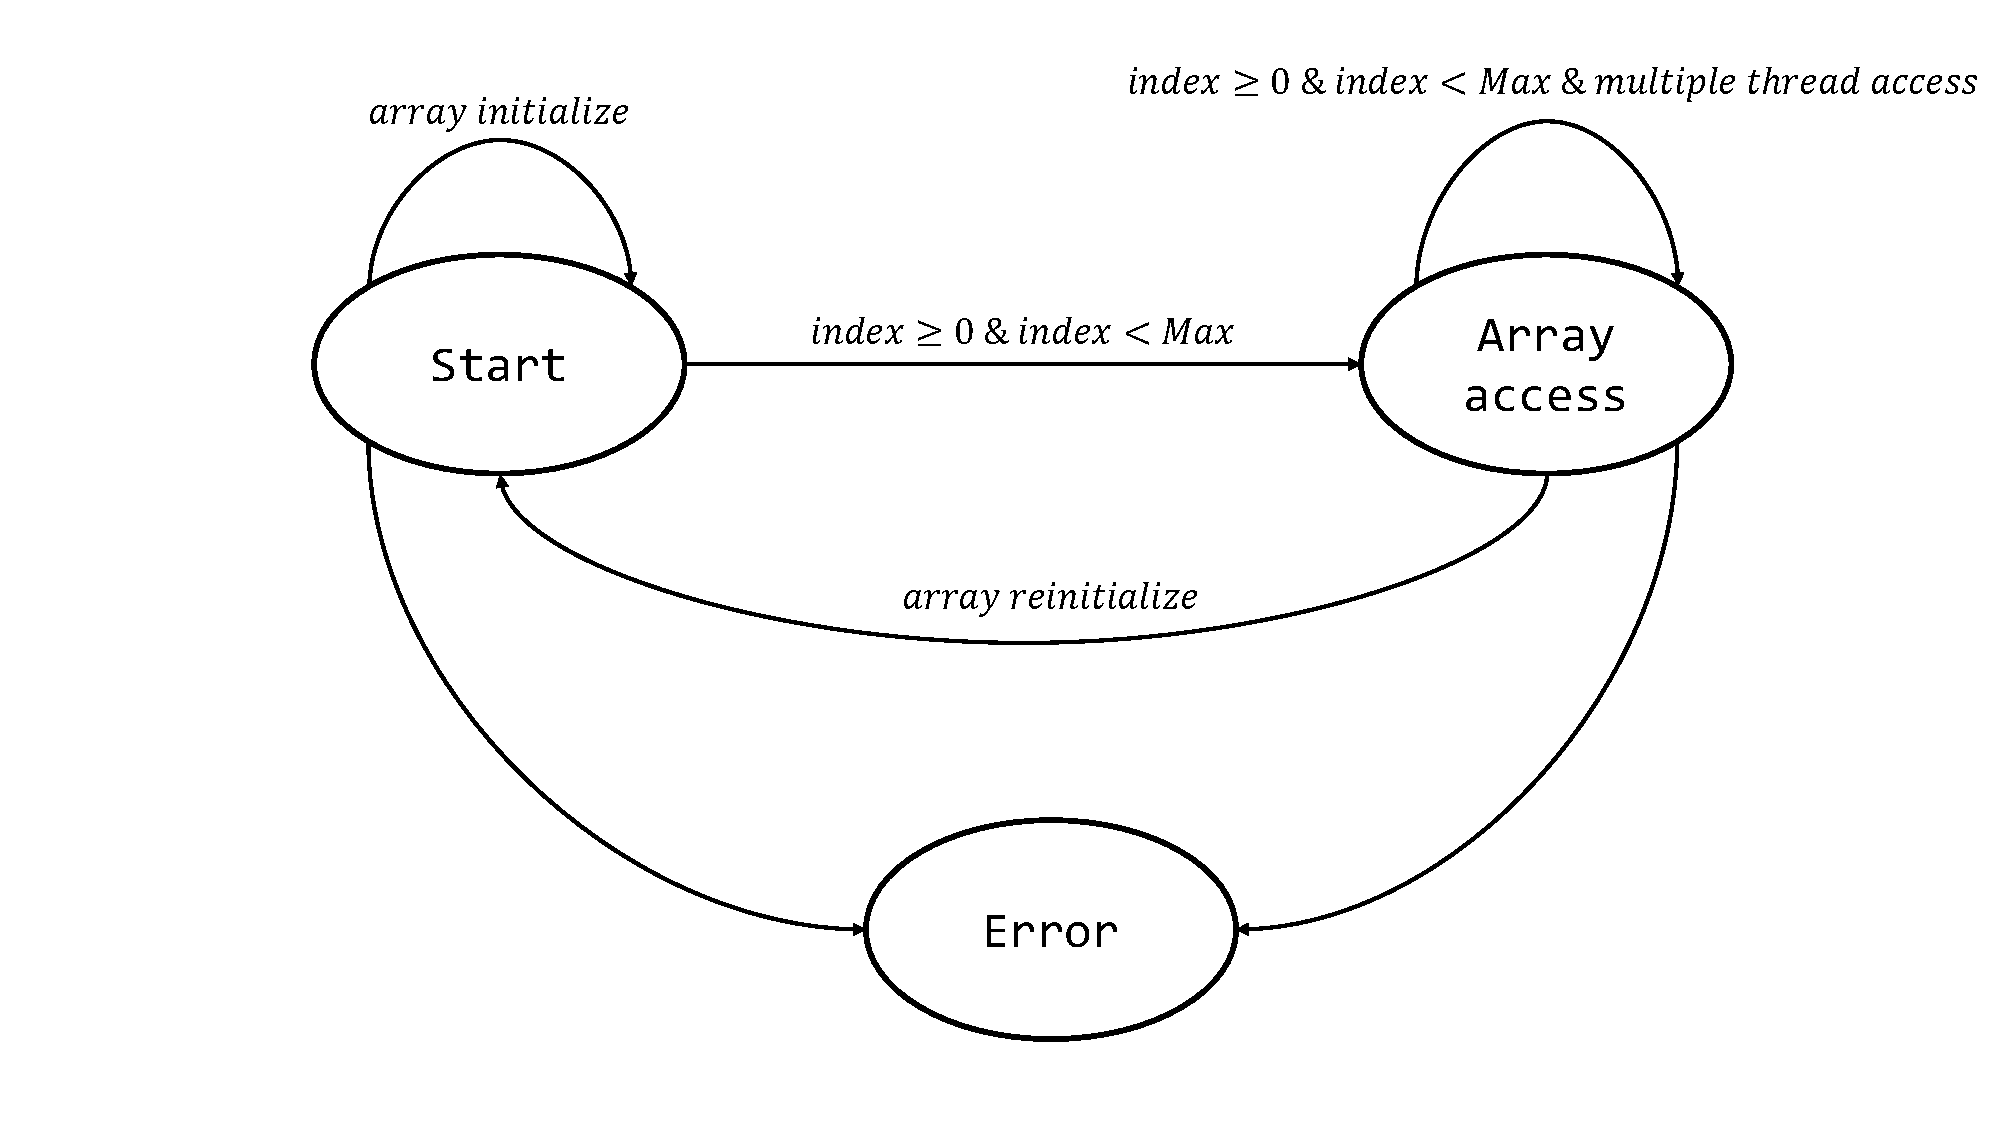
\includegraphics[width=0.65\textwidth]{images/ArrayIndex.pdf}
\caption{array index out of bound formulated as FSM }
\label{fig:array}
\end{figure}


We can visualize all runtime exceptions as finite state machine (FSM). When a
program violates such sequence, it throws runtime exception.
In Figure~\ref{fig:array}, array index out of bound (java.lang.
ArrayIndexOutOfBoundException) exception is described as a FSM.
Here, a program will be in safe bound as long as the $array\_index \geq 0$ or
$array\_index \leq max\_array\_size - 1$


%%%%%%%%%%%%%%%%%%%%%%%%%%%%%%%%%%%%%%%%%%%%%%%%%

%%%%%%%%%%%%%%%%%%%%%%%%%%%%%%%%%%%%%%%%%%%%%%%%%
%CallGraph consruction


\chapter{RepairingStrategy : Taint Analysis}
\label{chapter:callGraph}

We have used taint analysis to detect program paths between source-sink pair in
the program to determine which variables and objects go to tainted sink like
database, print stream, network stream etc. We have used InfoFlow framework and
modify it for our usage. The detaild design of the taint analysis module is
given in Chapter~\ref{chapter:SystemDesign}
Section~\ref{subsubsec:TaintingRule}. 

\section{Taint analysis : Definition}
\label{sec:TaintAnalysisDef}

The term \textbf{taint} in the aspect of programming language is defined as
below:
\begin{definition}
Set of variables which are associated with program input is the set of tainted
variables.
\end{definition}
\begin{definition}
Variables which are associated or referenced from tainted variables are also
tainted.
\end{definition}
So, the set of variables are called as \textbf{tainted variable set} which may
trigger some undesirable events in the application.

\section{Taint analysis : Taint Propagation}
\label{sec:TaintPropagation}

All tainted variables do not possess security threat. The tainted problem is
defined at three points. They are:

\begin{enumerate}
	\item Source descriptor $<m,n_s,p_s>$
	\item Derivation descriptor $<m,n_d,p_d>$
	\item Sink descriptor $<m,n_s,n_d,p_s,p_d>$
\end{enumerate}
Where $m$ is the method, $n$ is the number of parameter(s), $p$ is the access
path.$s$ and $d$ denotes to source and sink(destination) respectively.
\begin{figure}[ht!]
\centering
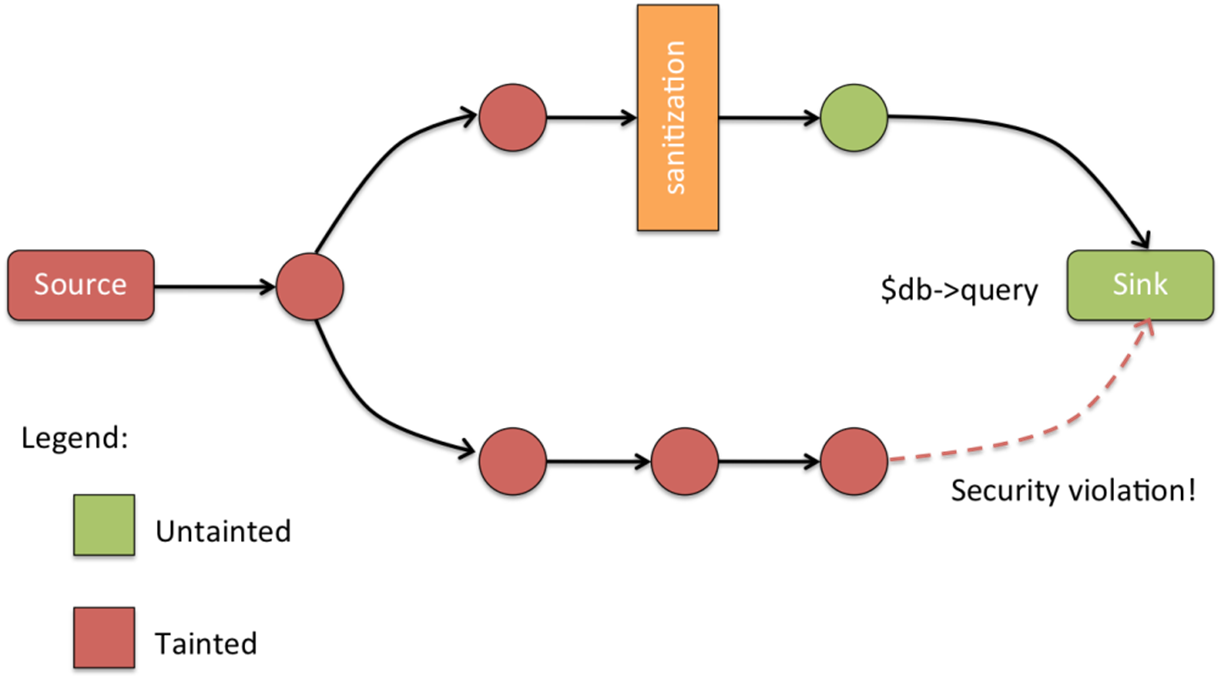
\includegraphics[width=5.5in]{images/Taint.png}
\caption{A simplified diagram indicating taint problem}
\label{fig:taint}
\end{figure}

\section{Taint Analysis : Relevance with Repairing Effort}
\label{sec:TaintRepairing}

We have considered static taint analysis of the program (here we are analyzing
only java byte code) to eliminate any possibility of patching on the statements
which may go to some tainted sink like database, print stream or network stream.
Doing such we can ensure that the variables and objects we are patching will be
contained inside the system thus will not be leaked to outside. On such example
can be a client application on which we have done patching. Assume that we
patched a string object which was given as a input to the program. Due to some
formatting problem, the program throws a runtime exception. Ins uch scenario we
will regenerate the string object according to the constraint in the program to
make sure it stays very close to a clean input string. in any case the generated
string goes out from the system and used as a input to any external module it
may causes problem as the patched sting was solely designed for that particular
program. 

To avoid such cases we analyze the statement which in in the path of potential
tainted source and sink. In such cases we would not patch such statements.

%%%%%%%%%%%%%%%%%%%%%%%%%%%%%%%%%%%%%%%%%%%%%%%%%

%%%%%%%%%%%%%%%%%%%%%%%%%%%%%%%%%%%%%%%%%%%%%%%%%
%Repairing Strategy


\chapter{Repairing Strategy : Exception Type}
\label{chapter:strgEx}

%marker
\textcolor{red}{\textbf{Please review this section}}\newline


\lstset{language=Java, caption=Java code which may throws runtime exceptions, label=example1}
\begin{lstlisting}

public class TestClass
{
	private int[] arr1;
	private int[] arr2;
	private int[] arr3;
		
	public TestClass(int[] arr1, int[] arr2, int[] arr3)
	{
		this.arr1 = arr1;
		this.arr2 = arr2;
		this.arr3 = arr3;
	}
	public int[] fun(int a, int b, int c, int d)
	{
		int temp0 = a + b;
		int temp1 = c * d;
		int temp2 = temp0 - temp1;
		//array index out of bound, negative index
		int temp3 = this.arr1[temp0];
		//array index out of bound, negative index
		int temp4 = this.arr2[temp1];
		//array index out of bound, negative index
		int temp5 = this.arr3[temp3];
		int temp6 = temp4 + temp5;
		int temp7 = temp6 - temp3;
		//array index out of bound, negative index, divide by zero
		this.arr1[temp6] = temp7/(d-a);
		//array index out of bound, negative index, divide by zero
		this.arr2[temp7] = temp7/temp4;
		if(arr2[temp1] ! = arr3[temp7])
			return arr1;
		else
			return null;
	}
}
public class MainClass 
{
	public void main(String[] a) 
	{
		int[] arr1 = {1,2,3,4};
		int[] arr2 = {1,2,3,4};
		int[] arr3 = {1,2,3,4};
		TestClass TC = new TestClass(arr1, arr2, arr3);
		int[] res = TC.fun(2,4,3,4);
		//Null pointer exception
		System.out.print("Result : "+res[2]);
	}    
}
\end{lstlisting}

In the Example~\ref{example1}, we have given a piece of java code which shows
multiple lines can throw several runtime exceptions.
In this example we consider three very common runtime exceptions:
NullPointerException, ArrayIndexOutOfBoundExcepltion, NegetiveIndexException,
ArithmeticException (i.e. divide-by-zero). In rest of this section, this
particular example will be used to demonstrate the repairing strategy.

\section{Static Analysis}
\label{subsec:symb}


\begin{figure}[htb]
\centering
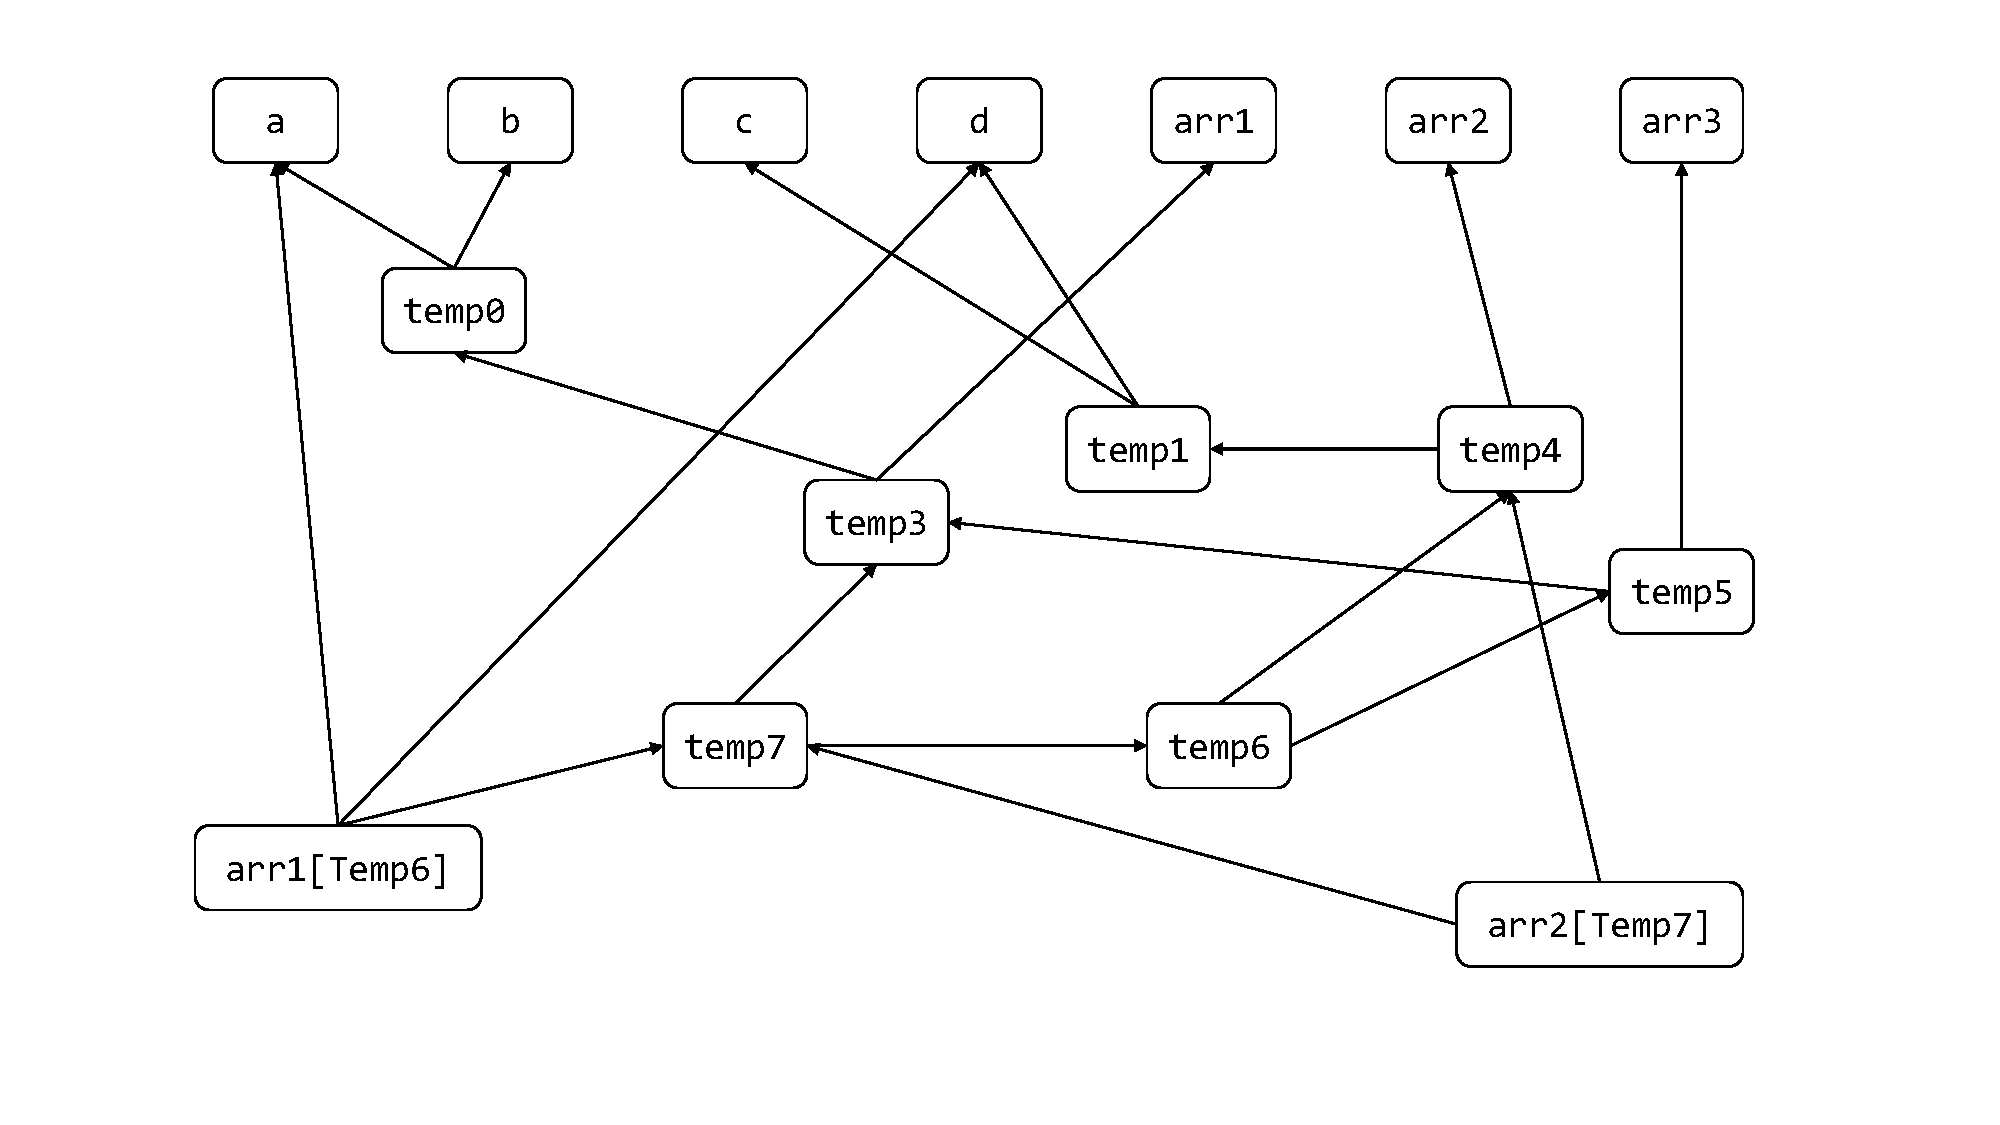
\includegraphics[width=4.8in]{images/depG.pdf}
\caption{Data dependency graph of the variables in code snippet~\ref{example1}}
\label{fig:datadep}
\end{figure}

We have done several  static analysis a priori  over the Java source code to
discover :
\begin{enumerate}
  
  \item Critical section of the code which are not eligible for patching. Eg.
  banking or any financial transaction which should be crashed in case of
  exception as suboptimal solution due to patching will led it to inconsistent
  state. This information will be available from the taint analysis module which
  will take place before the repairing module.
  
  \item We also analyze all the methods for method specific shilding as they can
  be called from the paths leading to both tainted sink and non tainted sink.
  The detailed description is available in Section~\ref{MethodShilding}.
  
  \item Static analysis of the program to discover potential points of failure and
  mark them.
  
  \item Build data dependency graph which will be used to generate appropriate
  code slice to be used as patch.
  In Figure~\ref{fig:datadep}, the data dependency graph of the
  code snippet~\ref{example1} is presented.
  
  \item The static analysis will also reveal which kind of exception is likely to
  happened at the time of execution.
  This information is necessary at the time of instrumenting the patch as it will
  determine the catch block.
  
\end{enumerate}

\section{Data set for Successful Program Runs}
\label{subsec:progrun}


\begin{figure}
\centering
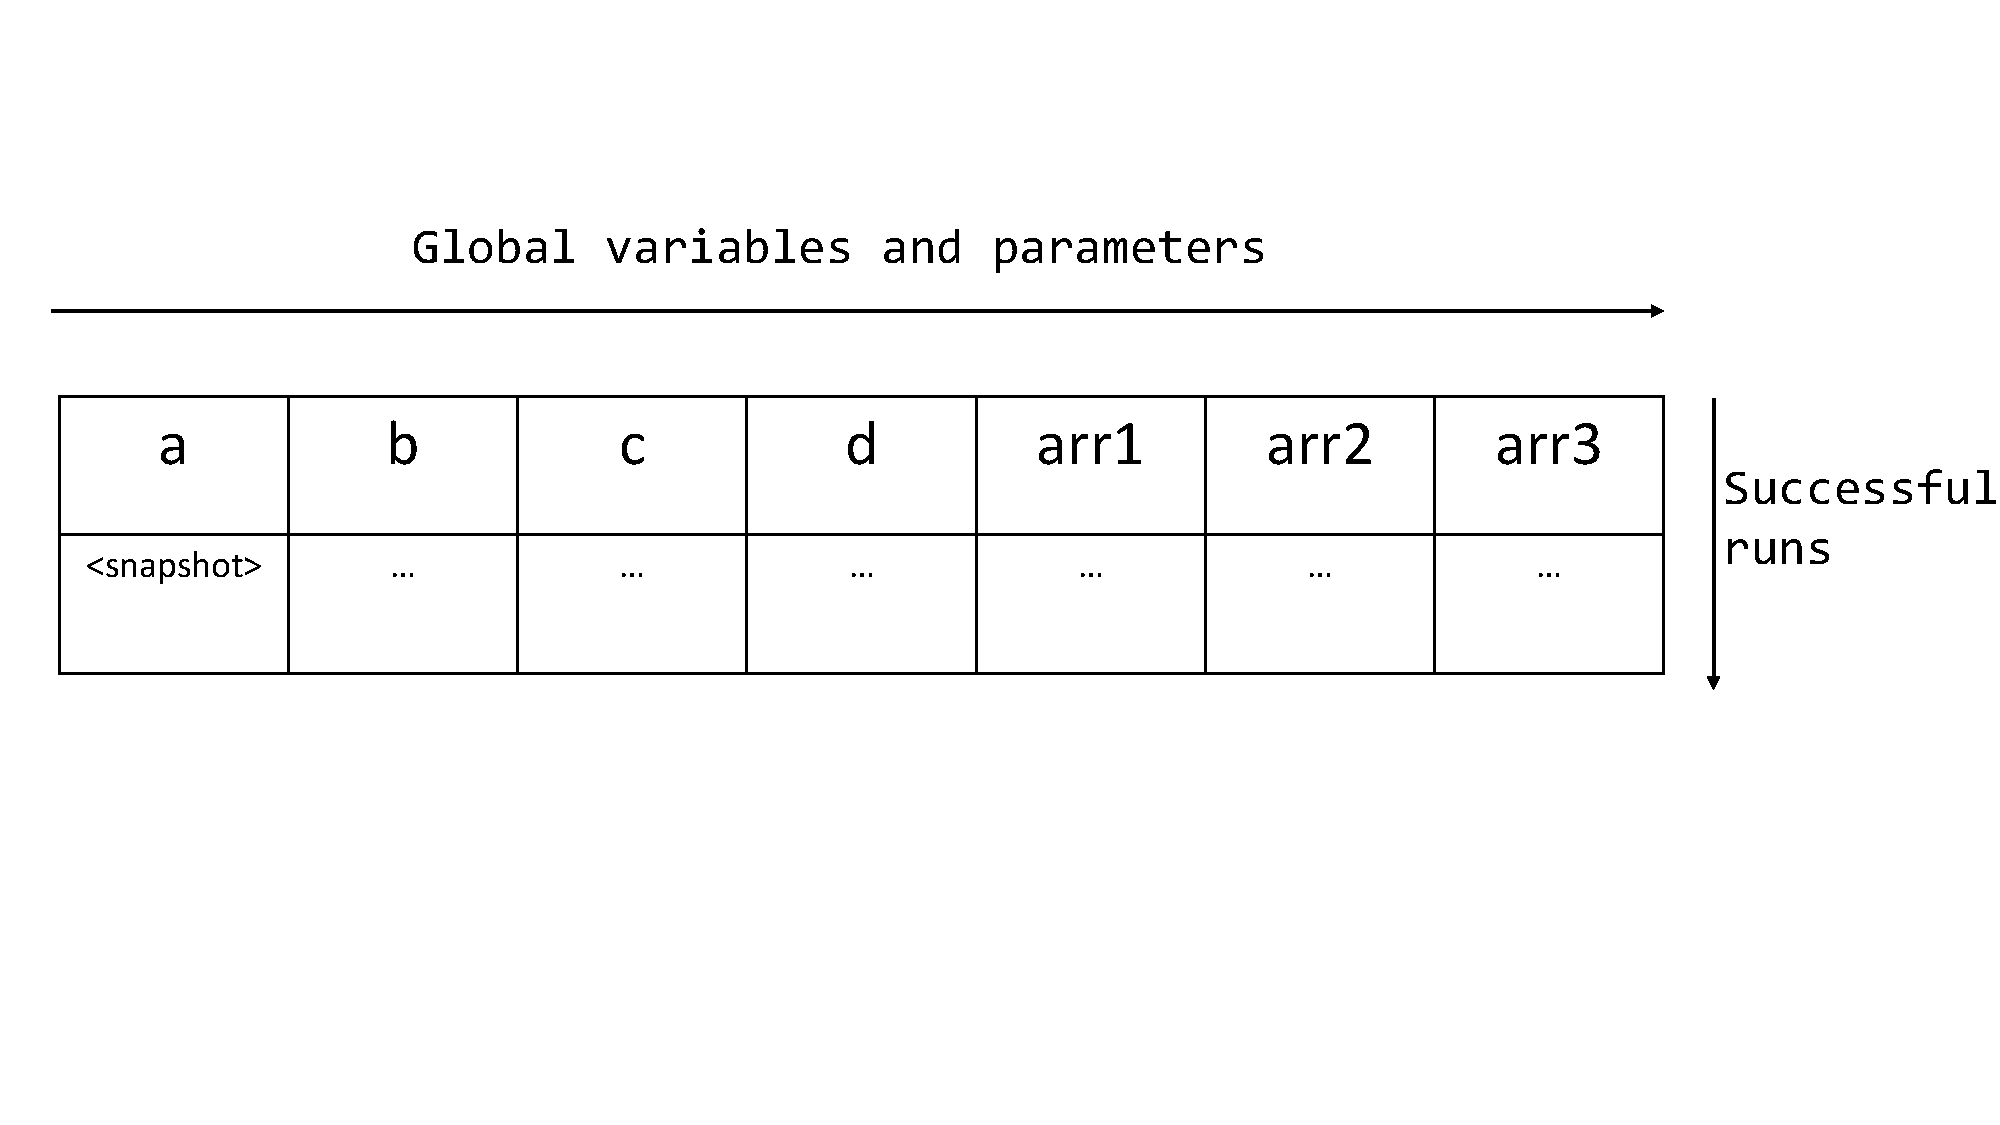
\includegraphics[width=4.8in]{images/succrun.pdf}
\caption{Indexed global variables and method arguments successful runs}
\label{fig:succrun}
\end{figure}

Here we stored all the traces of successful program runs.
Figure~\ref{fig:succrun} shows such indexed traces of all the global variables and method arguments. 
We store the snapshots of these objects. We won't store local variables as they can always be regenerated. 
As it is required to capture the snapshot of all these variable, we made deep cone of all of these objects and variables. 

%begin{table}[htb]
%\begin{tabular}{|c|c|c|c|c|c|c|}
%\hline
%a & b & c & d & arr1 & arr2 & arr3 \\ \hline
%\ldots & \ldots & \ldots & \ldots &	\ldots & \ldots & \ldots\\ \hline
%\end{tabular}
%\caption{Trace of successful runs}
%	\label{tab:Trace}
%\end{table}


\section{Matrices}
\label{subsec:martices}

%marker
\textcolor{red}{\textbf{Please review this section.}}\newline

\section{Instrumenting Patching}
\label{subsec:patchinstru}

We have used Soot framework which is a Java byte code manipulator to instrument patch. 
The patching technique is divided into two phases

\subsection{Determine Exception Type} 

At the time of execution, the exception may happened due to some specific values of some variables. We will catch the exception. Here the type of 
runtime exception is $java.lang.ArrayIndexOutOfBound$. This will be used to produce the try-catch block.
 
\subsection{Determine Optimal Code Slice}

The optimal code slice will be determined from the data dependency graph which was rendered at the time of static analysis mentioned in 
Section~\ref{subsec:symb}. In the code snippet~\ref{patchingexample1}, the example code snippet shows such code slice inside the catch block. 
As the error occurred at the line $int\ temp5\ =\ this.arr3[temp3];$ the statements which produces the temp3 and the statement which also 
involves $temp3$ or any other variables derived from $temp3$, would be included in the catch block for re-execution with the valued of the 
same from the data table of previous successful runs.

 
\onehalfspacing
\lstset{language=Java, caption=Patching code slice based on exception type,
label=patchingexample1}

\begin{lstlisting}

public class TestClass
{
	private int[] arr1;
	private int[] arr2;
	private int[] arr3;
		
	public TestClass(int[] arr1, int[] arr2, int[] arr3)
	{
		this.arr1 = arr1;
		this.arr2 = arr2;
		this.arr3 = arr3;
	}
	public int[] fun(int a, int b, int c, int d)
	{
		try
		{
		  int temp0 = a + b;
		  int temp1 = c * d;
		  int temp2 = temp0 - temp1;
		  int temp3 = this.arr1[temp0];
		  int temp4 = this.arr2[temp1];
	   //IndexOutOfBoundException as temp3 = 20
		  int temp5 = this.arr3[temp3];
		  int temp6 = temp4 + temp5;
		  int temp7 = temp6 - temp3;
		  this.arr1[temp6] = temp7/(d-a);
		  this.arr2[temp7] = temp7/temp4;
		}
		catch(IndexOutOfBoundsException indEx)
		{
		  int temp0 = a + b;
		  int temp1 = c * d;
		  int temp2 = temp0 - temp1;
		  int temp3 = this.arr1[temp0];
		//Bellow line is not part of the patch as 
		//temp1 and temp3are not related to temp3 
		//for which the exception occurred.
		  //int temp4 = this.arr2[temp1];
		  int temp5 = this.arr3[temp3];
		}
		if(arr2[temp1] ! = arr3[temp7])
			return arr1;
		else
			return null;
	}
}
public class MainClass 
{
	public void main(String[] a) 
	{
		int[] arr1 = {20,21,22,23};
		int[] arr2 = {1,2,3,4};
		int[] arr3 = {10,11,12,13};
		TestClass TC = new TestClass(arr1, arr2, arr3);
		int[] res = TC.fun(2,4,3,2);
		System.out.print("Result : "+res[2]);
	}    
}
\end{lstlisting}

\doublespacing

\section{Variable Tracking and Monitoring}
\label{subsec:taint}

\textcolor{red}{\textbf{I have added standard taint analysis technique here as an example. We can change it later}}\newline


Here we used taint analysis technique to tag variables and objects of our interest to monitor them. 
This steps are necessary as the values of the variables used during the instrumentation may cause further runtime exceptions. 
We used bit-vector which is an efficient technique to taint a object/variable. 
It requires maintain a single dimension byte array where each bit correspond to a single object/variable of our interest. 
The bit values will be flipped when it is required to taint ($1$) or untaint ($1$) an object/variable. 
We will only monitor these entities until all of them flushed from the program and the entire program reached to a stable state.


%%%%%%%%%%%%%%%%%%%%%%%%%%%%%%%%%%%%%%%%%%%%%%%%%

%%%%%%%%%%%%%%%%%%%%%%%%%%%%%%%%%%%%%%%%%%%%%%%%%
%Bounded Analysis


\chapter{Repairing Strategy : Bounded Forward and Backward Analysis}
\label{chapter:boundedAnalysis}

\section{Example Scenario}
\label{exampleScenario}

We have performed dataflow analysis by extending Soot main class. The objectives
of the dataflow analysis are the following:

\begin{itemize}
  \item For a target statement analyze used and defined variables.
  
  \item Extracts other statements which are both above and bellow the target
  statement in the control flow graph on which the used and defined variables
  are dependent on.
  
\end{itemize}

In the code snippet~\ref{snippet:dataflow}, we gave an example code based on java
\emph{String} API to demonstrate the analysis.

\onehalfspacing
\lstset{language=Java, caption=Dataflow analysis,
label=snippet:dataflow}
\begin{lstlisting}
void bar()
{
  foo("fname:lname");
}

String foo(String s)
{
  int a = s.indexof(":");
  int b = s.indexOf("&");
  int c = s.indexOf("#");
  int d = 0;
  if(c>0)
  {
    d = 1;
  }
  return s.substring(a,b);
}

\end{lstlisting}

Let us assume that our target is \texttt{s.substring(a,b)} which in this case
may throw an array index out of bound exception. In this target statement,
\texttt{a} and \texttt{b} are used variable which are dependent on another
String API method i.e \texttt{indexOf()} which calculates index of starting of a
sub-string or single character in the main string. In case the sub-string or the
character does not exist in the main string, \texttt{indexOf()} method returns
$-1$ which causes throwing a runtime exception in the \texttt{substring()}
method call.
\newline
By using dataflow analysis we try to understand how these different variables
are correlated and based on that how we can effectively apply patching technique
so the patching code will have very less footprint in the instrumented bytecode.
In the Section~\ref{subsec:boundedForward}, we have given detailed explanations
of such analysis.


\section{Flow Functions}
\label{sec:flowFunctions}

\begin{figure}[htb]
\centering
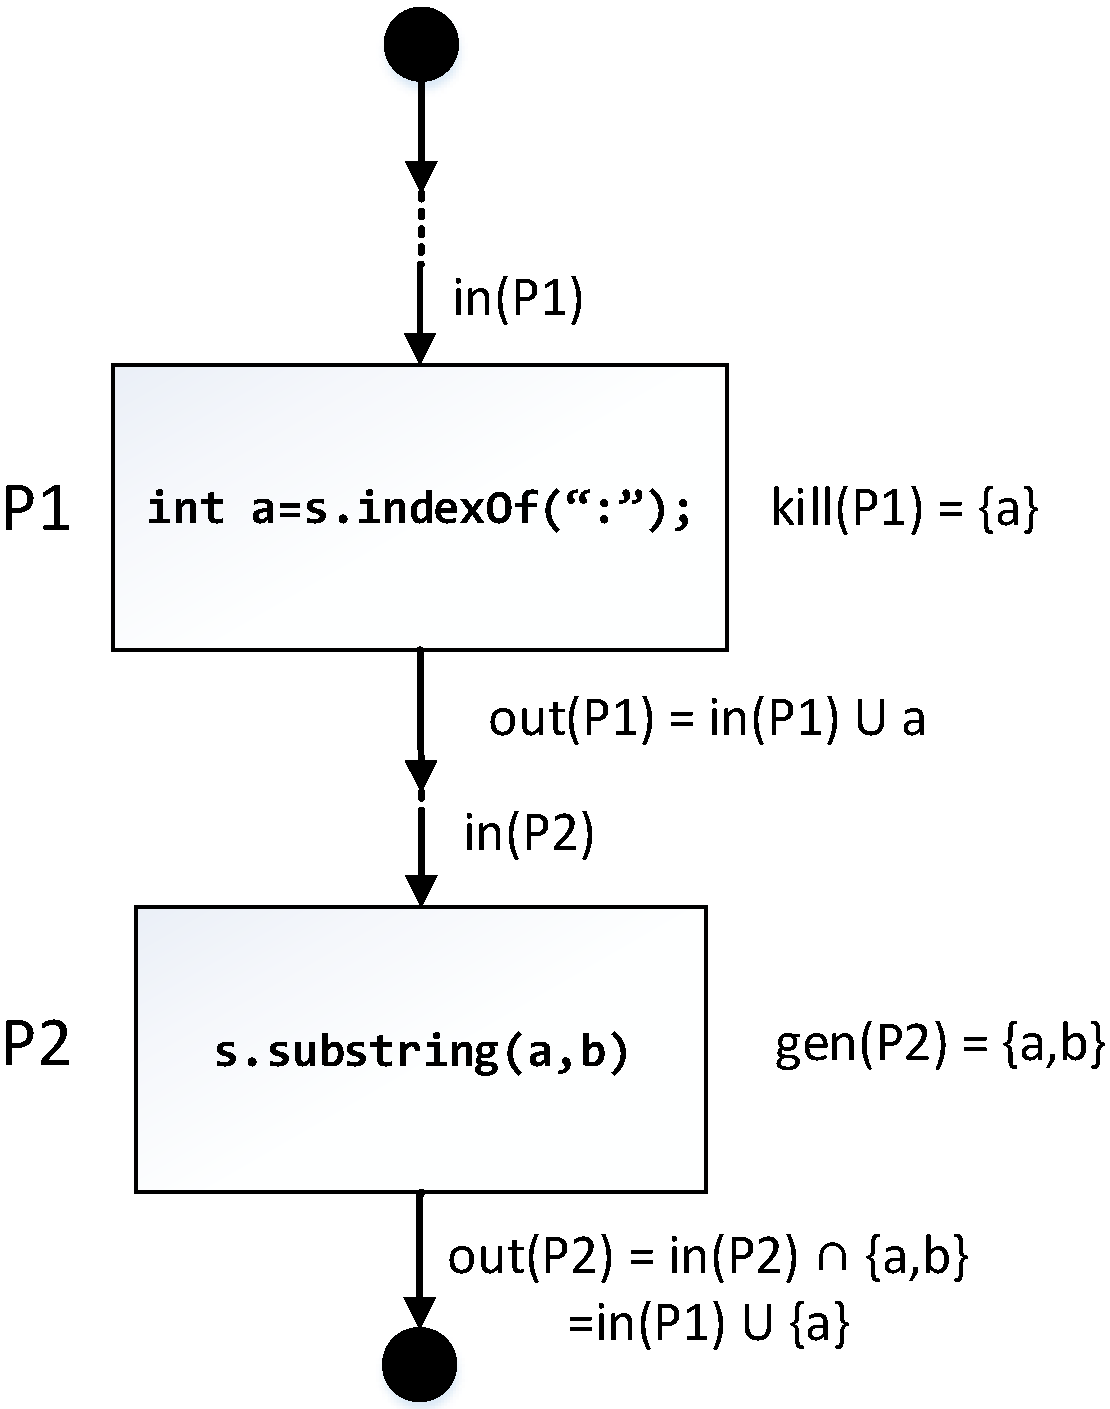
\includegraphics[width=3.2in]{images/dataflow.png}
\caption{Dataflow diagram with in, out set in forward analysis}
\label{fig:dataflow}
\end{figure}

\subsection{Bounded Forward Analysis}
\label{subsec:boundedForward}

Let us define $P_i$ as a program point/ node in the control flow graph. $in(P)$
and $out(P_i)$ respectively denotes in set and out set to and from the node $P$.
We define set $IG$ as the set of methods like \texttt{indexOf()},
\texttt{codePointAt()}, \texttt{CodePointBefore()} etc. which returns an integer
which can be used as input to other String methods. We also define set $IU$
which contains the methods which may use the integers produced by the methods in
$IG$ Then, 
$$out(P_i) = in(P_i) \cup Def(P_i)$$ where statement in P is a invoke statement
and method $m \in IG$ and
$$out(P_i) = in(P_i) \cap Used(P_i)$$ where statement in P is a invoke statement
and method $m \in IU$. Initial entry set = ${\phi}$.


We have defined $Def(P_i)$ set as the set of variables and objects which are
defined or redefined in the program point $P_i$. The set $Used(P_i)$ is also a
set of variables and objects which are used in the program point $P_i$.

\textbf{Example : } Consider the program statement \texttt{Pi : int a = b.fun(c
d)}.
Here the variable \texttt{a} is initialized, so $Def(P_i)$ = \texttt{\{a\}} and
as
\texttt{b, c, d} are used, $Used(P_i) =$ \texttt{\{b, c, d\}}

In the figure~\ref{fig:dataflow}, we gave an example of a sample CFG with in set
and out set.

\section{Constraint Satisfaction}
\label{sec:constraintSatisfaction}

Dataflow analysis plays an important role in preparing the patching. One
patching mechanism we have come up with \texttt{String} objects is tht by
solving constraints which may come up in future will produce patch of better
quality. More over, it is very easy to extend the solution to other objects type
based on their API and characteristics of conditions. One such example is given
in the following code snippet~\ref{snippet:constraintCheck}

\onehalfspacing
\lstset{language=Java, caption=Better patching mechanism with constraint
satisfaction, label = snippet:constraintCheck}
\begin{lstlisting}

void foo(String s, int i, int j)
{
	String str = s.substring(i,j);
	//some operation
	if(str.length() > 12){
	  //do something..
	}
	Integer in = 0;
	try{
	  StreamReader isr = new InputStreamReader(System.in);
	  String sin = new BufferedReader(isr).readLine();
	  in = Integer.parseInt(sin);
	}
	catch(IOException ex){}
	if(str.length() <= in){
	  //do something..
	}
	if(str.startsWith(SomeStringObject)){
	  //do something
	}
}

\end{lstlisting}

In the code snippet~\ref{snippet:constraintCheck}, the statement at line no $4$
is \texttt{s.substring(i,j)}, which can throw a
\texttt{IndexOutOfBoundsException}. This statement requires patching whic
involves generating a string for the object reference \texttt{str}. But in the
progrm, in line numbers \texttt{7, 16} and \texttt{20}, there are threee
conditional statements on \texttt{str} which involves constraint on the length
and the prefix of the string. There may be some set of constraint which can be
evaluated before hand, like the condition in in line numbers \texttt{7} which
involve a constant integer. But there can be cases like the conditional
statement in line numbers \texttt{16} which is also a lenght constraint like the
former, but in involves another variable which is taken frrom console, i.e. the
variable will be evaluated in run time. In such cases we can defer the
constraint evaluation process for that paricular condition. We can evaluate all
the conditions befor it, which can be safely evaluated. When we reach line
number \texttt{16}, then the variable \texttt{tt} would be available and can be
used to reevaluate the string \texttt{str}.

\subsection{Constraint Storage}
\label{subsec:constraintStorage}

For each of the string object, we store in the way illustrated in the
Figure~\ref{fig:constraint}.

\begin{figure}[htb]
\centering
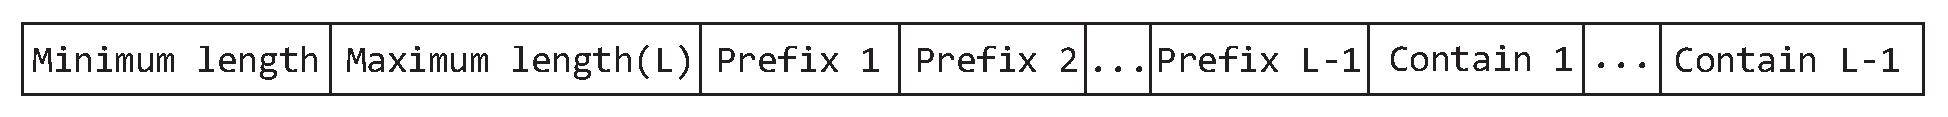
\includegraphics[width=6.5in]{images/constraint.eps}
\caption{String constraints storage format}
\label{fig:constraint}
\end{figure}

Wen to evaluate a new string object we need bounds like the minimuma and maximum
length, the prefixes and the candidate characters and their relative position.
We keep minimum information to safely evaluate the string.

\subsection{Constraint Evaluation Strategy}
\label{subsec:constraintStorage}

\begin{algorithm}
\DontPrintSemicolon
\KwData{String object $Str$ and constraint set $CS$.}
\KwResult{String object $Str$ such that $\forall i \in CS$, $Str$ satisfies $i$
}
\Begin
{
 $CS_{Str} \longleftarrow$ Get the constrint set for $Str$\;
 $MinLength \longleftarrow CS_{Str}[0]$\;
 $MaxLength \longleftarrow CS_{Str}[1]$\;
 $PrefixSet_{Str} \longleftarrow CS_{Str}[2 \rightarrow MaxLength + 1]$\;
 $ContainSet_{Str} \longleftarrow CS_{Str}[MaxLength +2  \rightarrow 2*MaxLength
 + 1]$\;
 
  \For{$C \in PrefixSet_{Str}$}
  {
   \If{$C$ is Empty}
   {
    continue\;
   }
   $PrefixLength \longleftarrow$ {\bf LENGTH OF} $C$\;
   
   \If{$PrefixLength$ is Maximum $\in PrefixSet_{Str}$}
   {
     Use $C$ to construct $Str$\;
   }
  }
 
  \For{$C \in ContainSet_{Str}$}
  {
   \If{$C$ is Empty {\bf OR} $C \in Str$}
   {
    continue\;
   }
   $Str \leftarrow Str$ {\bf APPEND} $C$\;
  }
  return $Str$\;
}
\caption{String object constraint evaluation}
 \label{algo:constraint}
\end{algorithm}

\subsection{Repairing Strategy using Constraint Evaluation}
\label{subsec:repairingStrategyConstraint}

The patching is evaluated in two ways, static and dynamic. We evaluated those
conditions which can be evaluated safely during compile time. Such constraints
have constants like \texttt{if(s.length<10)}. We looked for particular
constraints based on our storage specification 

%%%%%%%%%%%%%%%%%%%%%%%%%%%%%%%%%%%%%%%%%%%%%%%%%

%%%%%%%%%%%%%%%%%%%%%%%%%%%%%%%%%%%%%%%%%%%%%%%%%
%Constraint Automata
\doublespacing

\chapter{Repairing Strategy : Constraint Automata}
\label{chapter:strgCA}

\section{General Structure}
\label{subsec:generalCA}

\emph{Constraint automata} is a formalism to describe the behavior and possible
data flow in coordination models.
Mostly used for model checking. We have used it for the purpose of program
repairing technique. Here we define the finite state automata as follows :

$$(Q, \Sigma, \delta, q_0, F)$$
\begin{itemize}
\item $Q$: set of state where $|Q| = 2$, \emph{legal state}(init) and
\emph{illegal state} (error).
\item $\Sigma$: symbols, invariants based on exception type.
\item $\delta$: transition function. $init \rightarrow init$ is safe transition
and $init \rightarrow error$ is the invariant violation.
\item $q_0$: starting state, here $q_0 = init$.
\item $F$: end state, here it same as $q_0$.
\end{itemize}

\begin{figure}[!htb]
\centering
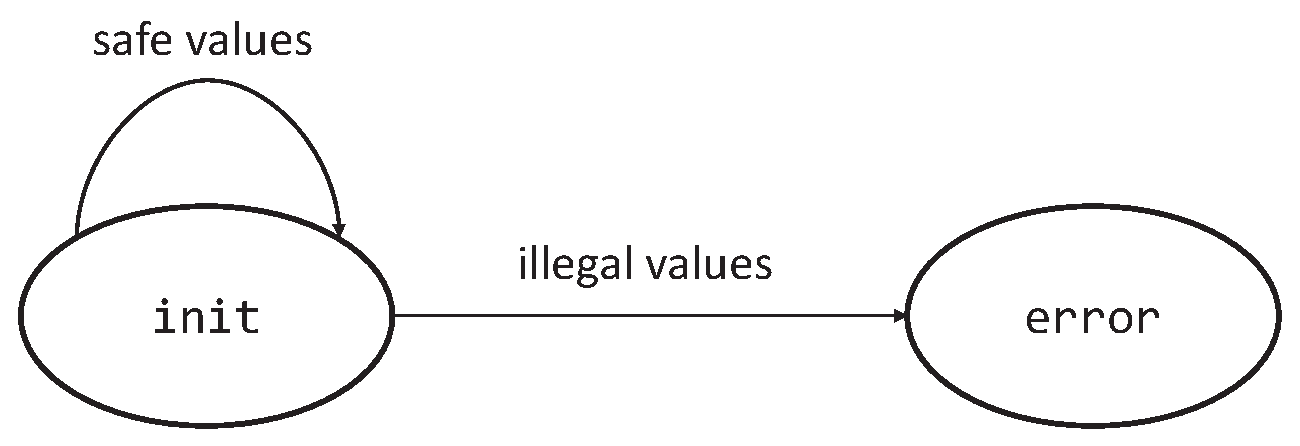
\includegraphics[width=3.2in]{images/automata.eps}
\caption{Constraint automata general model}
\label{fig:automata}
\end{figure}

According to the Figure~\ref{fig:automata}, the repairing mechanism will only
trigger when we have a transition from init state to error state due to
invariant violation.

\section{Patching Techniques}
\label{subsec:patchCA}

The patching technique is based on the exception type. We instrument the
patching code in a catch block keeping the original statement encapsulated in
try block.

\subsection{Array index out of bound exception}

Array index out of bound exception happen when one tries to access the array
with a index which is more than the size of the array or less than zero i.e.
with some negative value. We did the patching based on these two scenario.

\begin{itemize}
  \item When the index is more than the array size, we patch it by assigning
  $array.length - 1$.
  \item When the index value is less than $0$, then we patched it by assigning
  the ined to $0$.
\end{itemize}

In the code snippet~\ref{indexoutofbound} we show such example.


\onehalfspacing

\lstset{language=Java, caption=array index out of bound patching,
label=indexoutofbound}

\begin{lstlisting}
void foo()
{
  int []arr = {1,2,3,4};
  int index = 10;
  int y = 0;
  try
  {
    //original code
    y = arr[index];
  }
  //patching instrumentation
  catch(IndexOutOfBoundException ex)
  {
    if(index > arr.length)
      y = arr[arr.length - 1];
    else
      y = a[0];
  }
}

\end{lstlisting}

\doublespacing
\subsection{Negative Array Size Exception}

Negative array size exception occurs when one tries to create a array with a
negative size.
The patching is done based on data flow analysis. Suitable index size is
determined by looking at the successive statement dependent on the array.
To take a safe bound, we took maximum index size and set as the array size in
the new array statement~\ref{negativearraysize}.


\onehalfspacing
\lstset{language=Java, caption=arr index out of bound patching,
label=negativearraysize}

\begin{lstlisting}
void foo()
{
  int []arr = {1,2,3,4};
  int index = 10;
  int y = 0;
  try
  {
    //original code
    y = arr[index];
  }
  //patching instrumentation
  catch(IndexOutOfBoundException ex)
  {
    if(index > arr.length)
      y = arr[arr.length - 1];
    else
      y = a[0];
  }
}

\end{lstlisting}


\doublespacing
\subsection{Arithmetic Exception : Division-by-zero Exception}

Division by zero causes arithmetic exception. There are two different cases which were considered here. 
\begin{itemize}
 
 \item \textbf{Case I :} The denominator is going to the taint sink but the left
 hand side is not going to any taint sink.
 Here we will not manipulate the denominator as we are not manipulating any
 variable which are going to any taint sink.
 
 \item \textbf{Case II :} The denominator and the left hand side, both are not
 going to any taint sink. So they are safe to patch.

\end{itemize}

In the code snippet~\ref{divisionbyzero}, we demonstrate the patching technique
with an example java code.


\onehalfspacing
\lstset{language=Java, caption=arithmetic exception : division-by-zero patching,
label=divisionbyzero}

\begin{lstlisting}
void foo()
{
  int a = 10;
  int b = 0;
	int y;
  try
  {
    //original code
    y = a/b;
  }
  //patching instrumentation
  catch(ArithmeticException ex)
  {
    //case I
    if(taintSink(b))
      y = 0;
    //case II
    else
    {
      b = 1;
      y = a/b;
    }
  }
}
\end{lstlisting}


\doublespacing
\subsection{Null Pointer Exception}

Null pointer exception in Java is the most common runtime exception encountered. 
Thrown when an application attempts to use null in a case where an object is
required. There exists various scenarios where null pointer exception can
happen. These different scenario requires different patching techniques. Bellow
we enlist all cases and corresponding patching techniques.


\begin{itemize}
  \item \textbf{Case I} Calling the instance method of a null object. \newline
  \textbf{Patch :} This is patched~\ref{nullpointer1} by calling the
  constructor.
  In case there exists more than one constructor then we need to find most appropriate
  constructor. This is done by using data flow analysis in the successive
  statement to see which fields/methods been accessed and according to that
  most suitable constructor should be picked up, this will ensure safest way to
  deal with the later method calls/field accesses.
  

\onehalfspacing
\lstset{language=Java, caption=appropriate constructor, label=nullpointer1}

\begin{lstlisting}
class MyClass
{
 Integer field1;
 String field2;
 Double field3;

 public MyClass()
 {
  this.field1 = 1;
  this.field2 = null;
  this.field3 = null;
 } 
 public MyClass(Integer field1, String field2)
 {
  this.field1 = field1;
  this.field2 = field2;
  this.field3 = null;
 } 
 public MyClass(Integer field1, String field2, Double field3)
 {
  this.field1 = field1;
  this.field2 = field2;
  this.field3 = field3;
 }
 public Double getfield3()
 {
  return this.field3;
 }
}

class main
{
 Myclass mclass = null;
 Double a = null;
 try
 {
  //original code
  a = mclass.getfiled3() + 5.0;
 }
 //instrumentation
 catch(NullPointerException ex)
 {
  //choose appropriate constructor
  mlass = new MyClass(1, "a", 1.0); 
  a = mclass.getfiled3();
 }
}
\end{lstlisting}
 
 \doublespacing
  
  \item \textbf{Case II} Possible Accessing or modifying the field of a null
  object.\newline
  \textbf{Patch :} The patch is same as the previous one~\ref{nullpointer1}.
  
  \item \textbf{Case III} Taking the length of null as if it were an
  array.\newline
  \textbf{Patch :}The patch~\ref{nullpointer2} for this situation is very much
  similar to the negative array size exception. Here we will do a data-flow analysis to see all
  the successive statements where the array object has been used (read or
  write). For safety we will take the maximum index from those statements and
  reinitialize the array object with the size.


\onehalfspacing    
\lstset{language=Java, caption=array null pointer exception,
  label=nullpointer2}

\begin{lstlisting}
int[] bar(int a)
{
 int []arr = new int[a];
 int []b = (a > 10) ? arr:null;
 return b; 
}
void foo()
{
 int[] arr;
 int []arr = bar(5);
 try
 {
  //access or modify any field of arr
  //this will throw a null pointer exception
 }
 //instrumented code
 catch
 {
  int ARRAY_SIZE = 11;
  int []arr = new int[ARRAY_SIZE];
  //access or modify any field of arr
 }
}
\end{lstlisting}

\doublespacing
  \item \textbf{Case IV} Accessing or modifying the slots of null as if it were
  an array.
 \textbf{Patch :} The patching mechanism is exactly same as
 before~\ref{nullpointer2}.
 
  \item \textbf{Case V} Throwing null as if it were a Throwable value.
\end{itemize}


%%%%%%%%%%%%%%%%%%%%%%%%%%%%%%%%%%%%%%%%%%%%%%%%%

%%%%%%%%%%%%%%%%%%%%%%%%%%%%%%%%%%%%%%%%%%%%%%%%%
%Design of the System
\doublespacing

\chapter{\tool : Design of the System}
\label{chapter:design}

\section{Goals}
\label{sec:tool:goals}

We identify the broad design goals for a technique to automatically repair
malformed strings or incorrect handling of strings as follows:

% i) identifies the statements which might be vulnerable to string-related errors,
% and are less critical to the functionality of the application such that
% suboptimal behavior might be acceptable,
% iii) generates patches by identifying constraints on the string data and if
% required, tweaks \code{String} API  parameters to regenerate legally correct
% string data,
% iv) optimizes the number of statements to be patched by retaining only the ones
% that need to be protected,  

\myparagraph{(i) High patch fidelity} We require that the patched program must
preserve the intended program behavior, \ie\ the patch must be precise, and
should not induce any undesirable control flows in the repaired program.

\myparagraph{(ii) Non-invasive instrumentation} We require that the technique
must ensure no side-effects (aside from optimally repairing objects) during
normal program execution, and activate patches only when the program is
guaranteed to crash.

\myparagraph{(iii) Low system overhead} We desire that the patched program must
incur no runtime overhead during normal program execution, and only negligible
overhead in case of failures.

\section{Design}
\label{sec:tool:design}

\begin{figure}[t] \centering
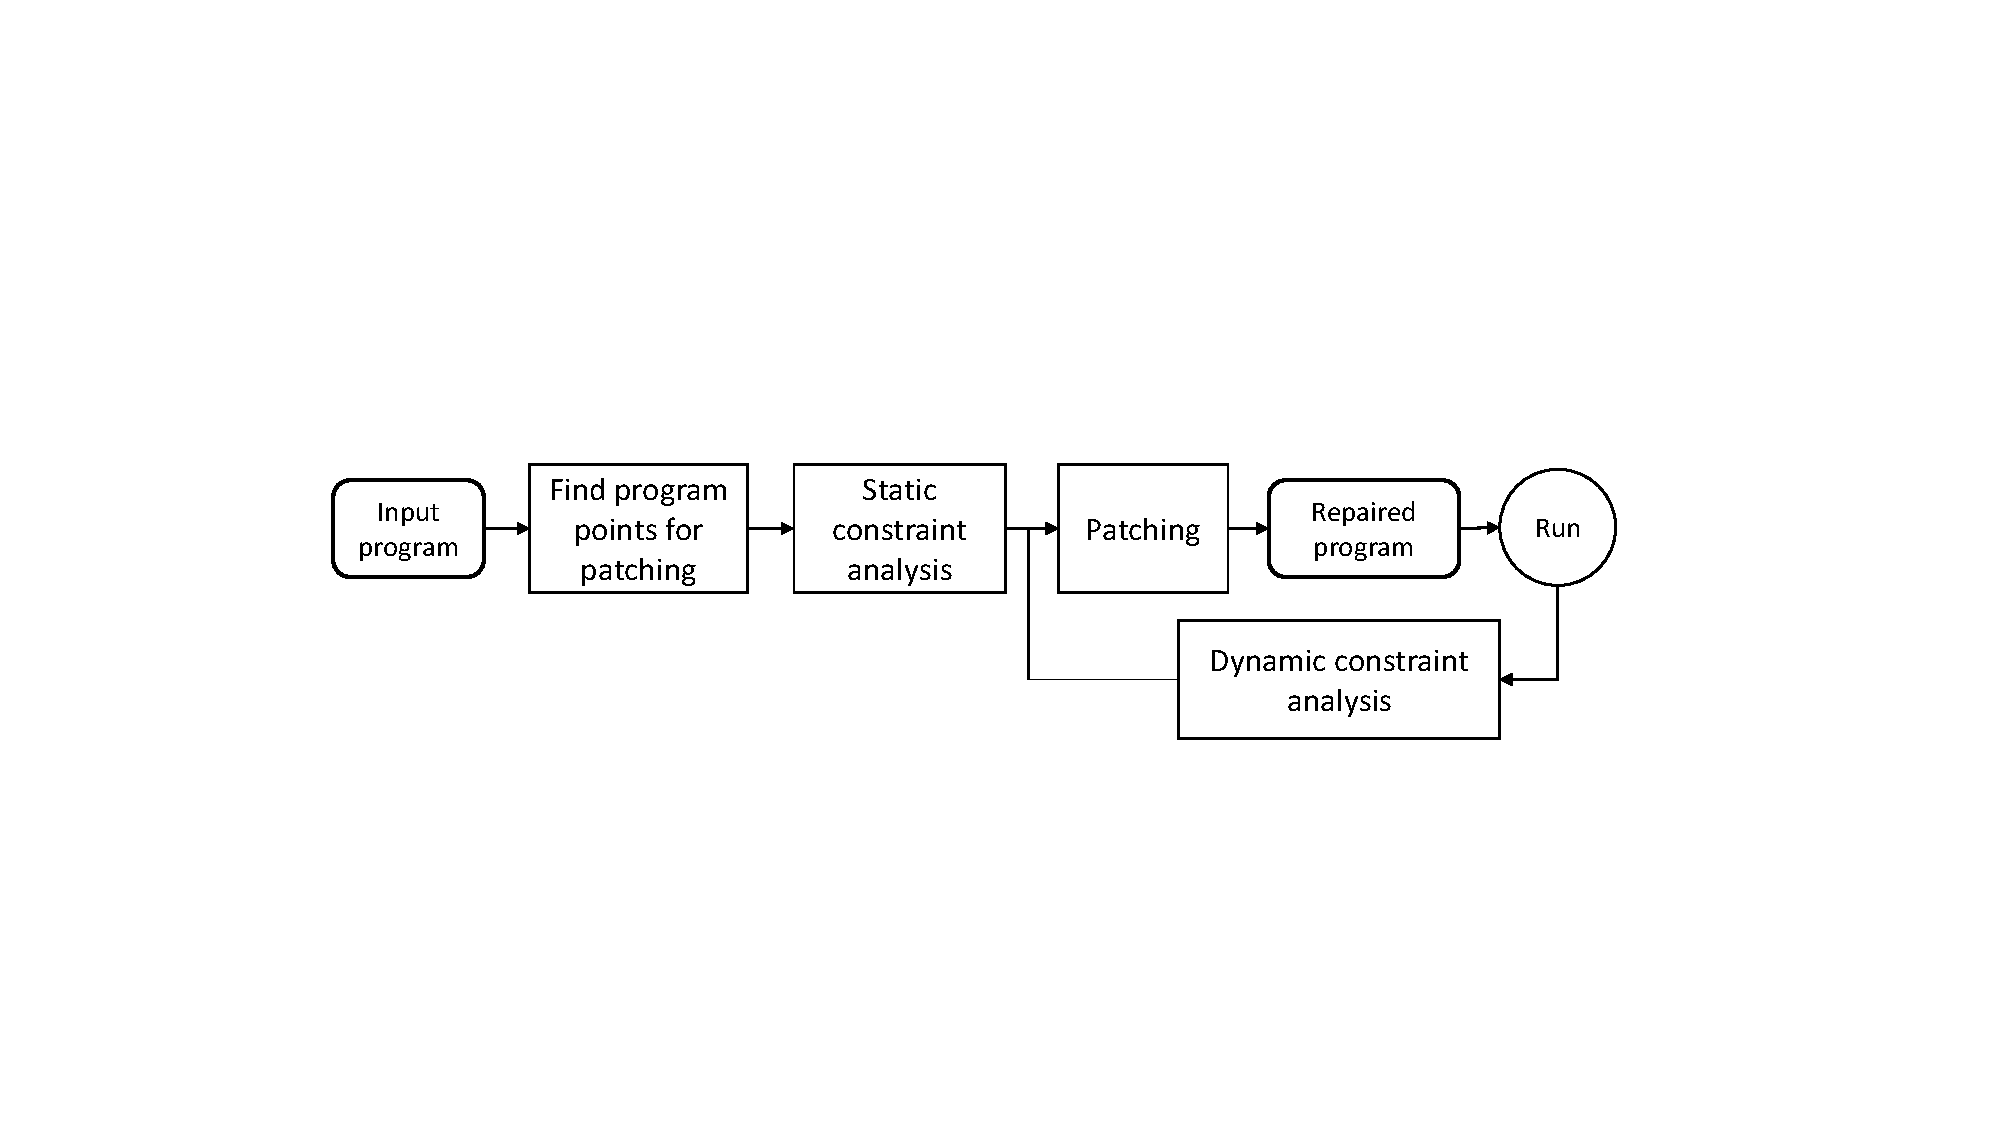
\includegraphics[scale=.6]{images/NewDesignDiagram.pdf}
\caption{\tool\ workflow.}
\label{fig:overallDesign}
\end{figure}

\myparagraph{\underline{Key Idea}} \tool\ leverages a combination of program 
analysis techniques to precisely identify program instrumentation points, and
builds upon custom algorithms to generate targeted, high quality patches for
repairing programs with potential runtime exceptions, while still satisfying
goals mentioned in \xref{sec:tool:goals}.

Figure~\ref{fig:overallDesign} shows \tool's workflow, which involves three
main stages. First, \tool\ uses program analysis techniques to precisely
identify points of interest, \ie\ string objects or API arguments that must be
repaired to prevent runtime exceptions. In the second stage, \tool\ leverages
custom algorithms to generate relevant patches. Specifically, \tool\ performs
intra-procedural static and dynamic analyses to identify and evaluate
constraints on the string objects under consideration. Third, \tool\ uses the
constraints evaluated in the earlier stage to programatically generate and embed
patches inside \texttt{catch} blocks to ensure that they do not get activated
during normal program execution.

\subsection{Precise Identification of Instrumentation Points: }
\label{sec:tool:stage1}

\begin{figure}[t] \centering
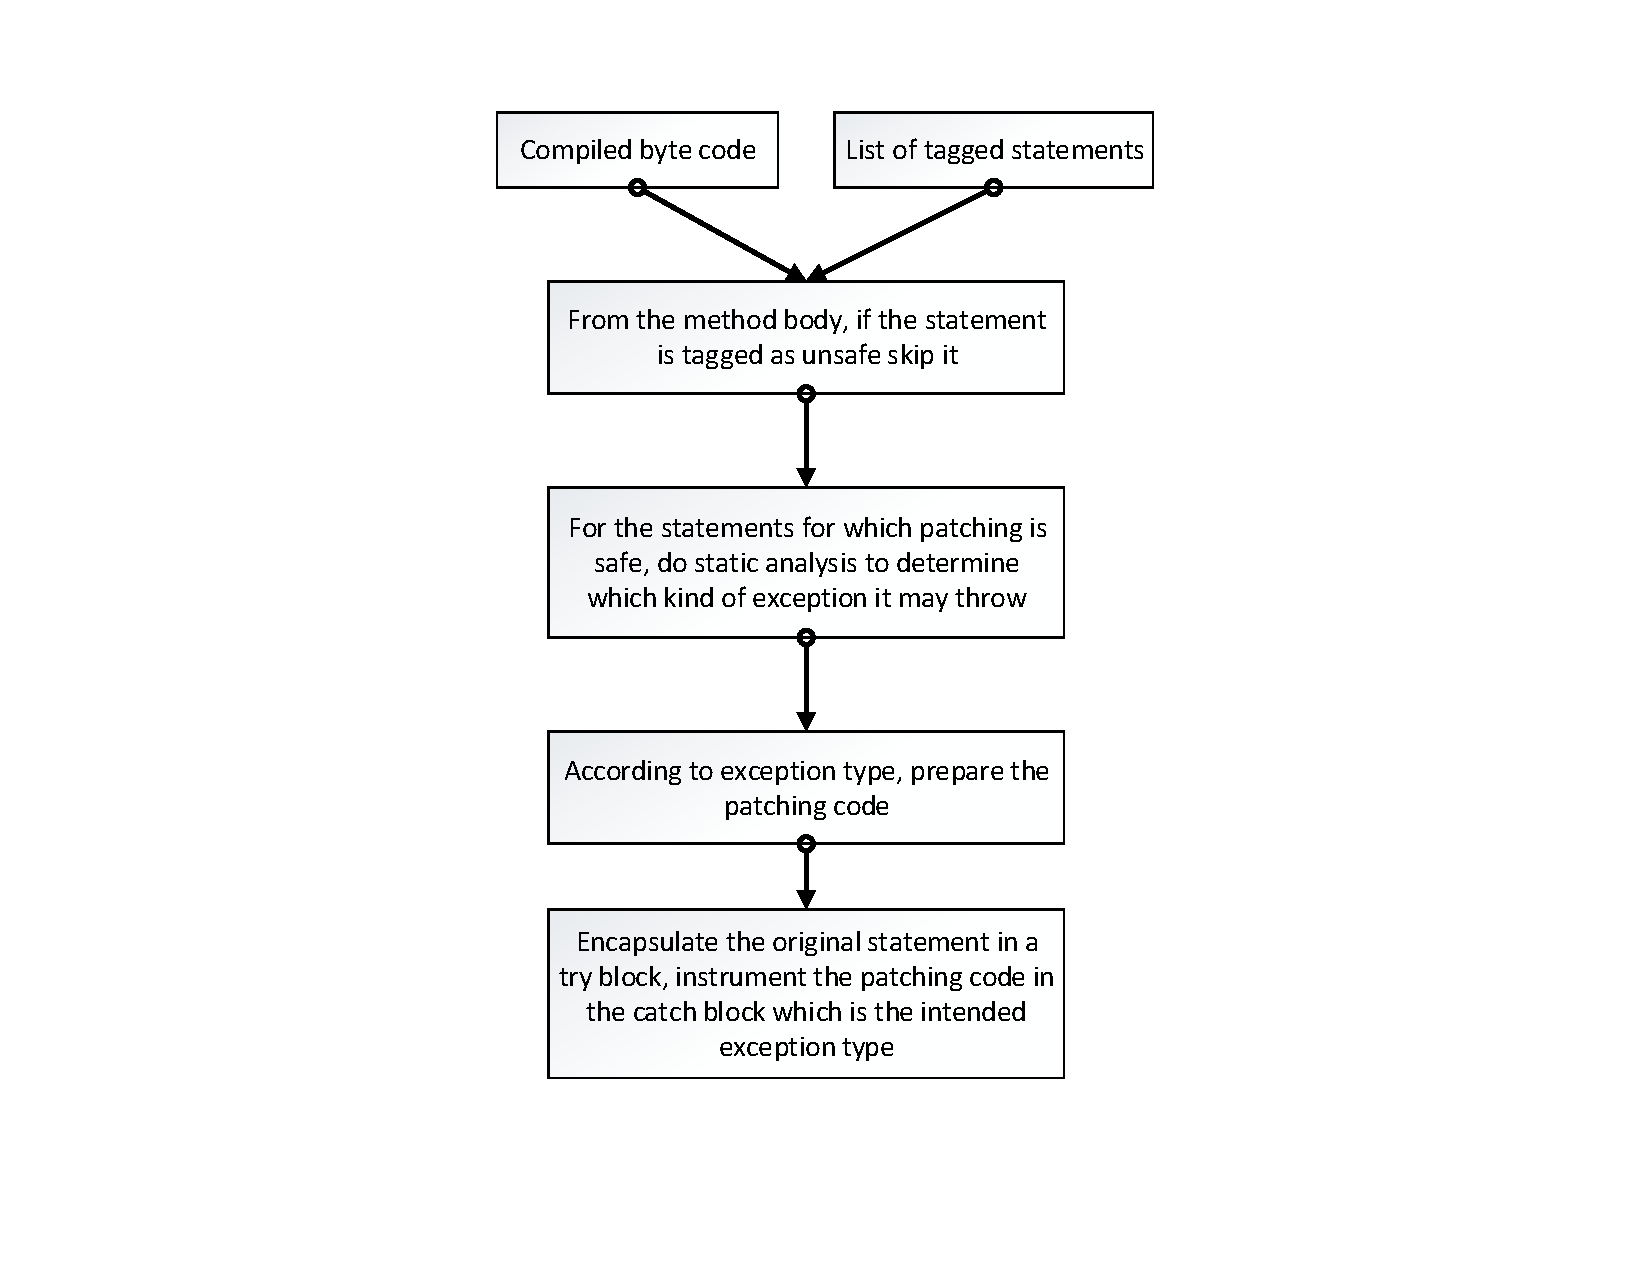
\includegraphics[scale=.5]{images/PatchModule.pdf}
\caption{\tool\ Patch module flow diagram}
\label{fig:overallDesign}
\end{figure}



In this stage, \tool\ leverages a combination of program analyses to accurately
determine the minimum set of points of interest where instrumentation is
required to repair. We list several techniques below that help \tool\ achieve
precision.

\myparagraph{(i) Taint analysis} The main purpose of taint analysis is to
broadly identify which program statements can be patched (possibly even
suboptimally) without affecting the program control flow, \ie\ affect only
objects that are generated and stay within the application throughout their
lifetime. While this principle is not a binding constraint, it ensures that
\tool's repairing mechanism does not adversely affect critical program behavior.
We specify a generic set of sensitive sources and sensitive sinks for each input
program, to identify critical program paths where a repaired \code{String}
objects (and thus possibly suboptimal) must not flow. For example, \tool\ does
not repair program statements that lie along a control flow path that leads to
an I/O sink, like file system, console, network, GUI, etc.

\begin{table}[t]
\centering
% \setlength{\tabcolsep}{3pt}
\begin{tabular}{|l|l|}
\hline
\multicolumn{1}{|c|}{\textbf{Class}} & \multicolumn{1}{c|}{\textbf{Source}}\\
\hline
\code{java.io.InputStream} & \code{read()}\\
\code{java.io.BufferedReader} & \code{readLine()}\\
\code{java.net.URL} & \code{openConnection()}\\
\code{java.util.Scanner} & \code{next()}\\
% \code{javax.servlet.http.HttpServletRequest} & \code{getParameter()}\\
\code{javax.servlet.ServletRequest} & \code{getParameter()}\\
\code{org.apache.http.HttpResponse} & \code{getEntity()}\\
\code{org.apache.http.util.EntityUtils} & \code{toString()}\\
\code{org.apache.http.util.EntityUtils} & \code{toByteArray()}\\
\code{org.apache.http.util.EntityUtils} & \code{getContentCharSet()}\\
\hline
\end{tabular}
\caption{Common sensitive sources in \java.}
\label{table:TaintSources}
\end{table}

\begin{table}[t]
\centering
% \setlength{\tabcolsep}{3pt}
\begin{tabular}{|l|l|}
\hline
\multicolumn{1}{|c|}{\textbf{Class}} & \multicolumn{1}{c|}{\textbf{Sink}}\\
\hline
\code{java.io.FileOutputStream} & \code{write()}\\
\code{java.io.OutputStream} & \code{write()}\\
\code{java.io.PrintStream} & \code{printf()}\\
\code{java.net.Socket} & \code{connect()}\\
\code{java.io.Writer} & \code{write()}\\
\hline
\end{tabular}
\caption{Common sensitive sinks in \java.}
\label{table:TaintSinks}
\end{table}

The taint analysis module take as input the compiled byte code intended to be
repaired, and generates a control flow graph identifying program statements that
lie along paths from sensitive sources to sensitive sinks. Since, \tool\ targets
strings in particular, it must support taint propagation for all \java\ APIs
that support string manipulation, including \code{StringBuffer} and
\code{StringBuilder}. All \code{String} objects (whether generated or assigned)
that lie along the tainted path from a sensitive source to a sensitive sink are
marked as \textit{unsafe} to patch. Subsequently, \tool\ does not repair such
\code{String} objects. Tables~\ref{table:TaintSources} and
\ref{table:TaintSinks} list some common sensitive sources and sinks for several
classes in \java.

\myparagraph{(ii) Call graph analysis} \tool\ leverages call graph analysis to
further improve the precision for finding instrumentation points. Although
unlikely, it is possible that the developers may themselves handle code that
raises runtime exceptions. Thus, \tool\ must not instrument program points that
are explicitly handled by the developers, since repairing such statements
would definitely alter the intended control flow.

Checked runtime exceptions may be placed in the (i) same method, or (ii)
upstream in the call chain. While handling the former scenario is trivial,
\tool\ handles the latter case by identifying all possible call chains (in
the call graph) involving the concerned method using reverse Breadth First
search (BFS), and determines ancestor methods where the call site was wrapped in
\code{try-catch} block of compatible exception type or not.

\myparagraph{(iii) Reaching definitions analysis} Taint and call graph analyses
together provide a set of program points to be instrumented with the
patch. However, this set can be further pruned. \tool\ performs \textit{reaching
definitions} analysis to skip marked statements if
(i) the string variables contained in such statements have already been patched
upstream in the method, and (ii) the variables have not been redefined along any
path that originates from the patched statement. This analysis further reduces
instrumentation points in a program.

\subsection{Patch Generation: }
\label{sec:tool:stage2}
% 
The output from the first stage is essentially a set of program points,
typically bytecodes or some other intermediate representation, denoting
\code{String} objects or APIs that are safe to repair. Once these
instrumentation points have been identified, \tool\ determines the
possible patches that can be applied to each of them. Specifically, a program
patch constitutes a set of constraints on either the \code{String} object or the
parameters to the \code{String} API under consideration, such that the new
repaired \code{String} object that is generated will satisfy all constraints and
thus the patched program does not throw any runtime exceptions.

\tool's patch generation mechanism involves two main parts (i) constraint
collection and evaluation, and (ii) code generation. We now describe \tool's
patch generation mechanism in detail. 

%
\begin{figure}[t]
\centering
%% change the font size in the img; make it min len, max len
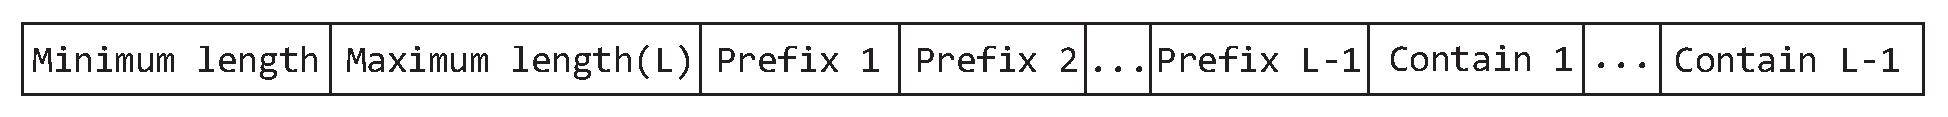
\includegraphics[width=\linewidth]{images/constraint.eps}
\caption{Constraints involving Strings.}
\label{fig:constraint}
\end{figure}
% 

\myparagraph{Constraint collection and evaluation} \tool\ leverages a hybrid
approach to collect all possible constraints that must be satisfied, and thus
generates a high quality patch to repair the program. A constraint on a string
object is defined as a set of permissible values that can uniquely define the
string. \tool\ uses a simple constraint set that includes minimum and maximum
length, along with set of permissible prefixes and substrings, as shown in
Figure~\ref{fig:constraint}.

\begin{algorithm}[t]
\DontPrintSemicolon
\KwData{Control flow graph $CFG$ for program $P$}
\KwResult{Patched program $\hat{P}$}
\Begin
{
 \For{$\forall$ node $N \in CFG$} {
  Statement $S$ in node $N$\\
  \lIf{$S$ contains \code{String} API call} {\\
  	\mytab $str \longleftarrow$ \code{String} reference on $S$
  	
  	\lIf{$S$ can throw \code{RuntimeException}} {\\
  	  \mytab Exception class $EC \longleftarrow$ \code{RuntimeException} of
$S$\\
          \mytab $CES_{str} \longleftarrow$ all conditional statement in $P$ on
$str$\\
  	  \mytab $CS_{str} \longleftarrow$ output of
Algorithm~\ref{algo:constraintCollection}$(CES_{str})$\\

  		\mytab \lIf{$str$ have sufficient constraints in $CS_{str}$} {\\
			\mytab \mytab \code{/* Static constraint analysis */}\\
  			\mytab \mytab $str \longleftarrow$ output of
Algorithm~\ref{algo:constraint}$(CS_{str})$
  		} \mytab \lElseIf {$str$ encountered exception} {\\
  		        \mytab \mytab \code{/* Dynamic constraint analysis */}\\
  		        \mytab \mytab $CS_{str} \longleftarrow$ output of
Algorithm~\ref{algo:constraintCollection}$(CES_{str})$\\

                        \mytab \mytab \lIf{$str$ have sufficient constraints in
$CS_{str}$} {\\
                        \mytab \mytab \mytab $str \longleftarrow$ output of
Algorithm~\ref{algo:constraint}$(CS_{str})$
  		} \mytab \mytab \lElse {\\
  		        \mytab \mytab \mytab $str \longleftarrow$ output of
Algorithm~\ref{algo:stringPatchParametr}$(S)$
  		}\vspace{-4em}
	}
    }
  }
 }
}
\caption{Patching strategy for \code{String} objects.}
\label{algo:patchingStrategy}
\end{algorithm}

The hybrid approach has a static component that makes a forward pass over the
program to collect declarative constraints on string objects, such as their
length or prefix, etc. \tool\ invokes the dynamic component if there are constraints
such that the constraint set cannot be evaluated. In
such scenarios \tool\ (i) generates a patch that itself dynamically collects
constraint information, (ii) augments it with the previously collected static
constraint details, and (iii) evaluates these constraints on the fly to generate
repaired \code{String} objects, which do not cause the program to throw runtime
exceptions. Algorithm~\ref{algo:patchingStrategy} gives an overview of this
hybrid approach.

\begin{algorithm}[t]
\DontPrintSemicolon
\KwData{Set of conditional statement on string $str$}
\KwResult{Constraint set $CS_{str}$}
\Begin
{
  \For{Conditional statement$ \leftarrow i$, $\forall i \in CS_{str}$}
  {
   $i \Rightarrow str\ *\ OP$ \code{/*where $*$ is the binary operator*/}\\
   \lIf{$*$ is $==$} {\\
   \mytab $maxlength_{str} \longleftarrow OP$\\
   \mytab $minlength_{str} \longleftarrow OP$
   } \lElseIf {$*$ is $\textgreater$ {\bf AND} $*$ is $\ge$} {
    $minlength_{str} \longleftarrow OP$
   } \lElseIf {$*$ is $\textless$ {\bf AND} $*$ is $\le$} {
    $maxlength_{str} \longleftarrow OP$
   } \lElseIf {$*$ is Prefix Check} {
    $\textit{PrefixSet}_{str} \cup OP$
   } \lElseIf {$*$ is Contains Check} {
    $\textit{ContainSet}_{str} \cup OP$
   }
  }
}
\caption{Constraint collection for \code{String} objects.}
\label{algo:constraintCollection}
\end{algorithm}

\begin{itemize}

 \item \textbf{Static constraint collection}: \tool's static constraint
collection phase identifies all declarative constraints.
Algorithm~\ref{algo:constraintCollection} briefly describes the steps to
populate the constraint store shown in Figure~\ref{fig:constraint}.
Specifically, \tool\ iterates over all program code and analyzes conditional
statements involving string objects of the form \code{if (st.length() == $5$)}.
\tool\ considers only those constraints that the object must satisfy to ensure
that the control flows through the \textit{preferred} branch of the conditional.
We define the preferred branch as the one that does not throw exceptions or
error conditions, like \code{System.err.print()}. In other words, \tool\ only
considers the conditional expressions in the branches that do not involve any
exceptions or error paths. Note that \tool\ also evaluates $OP$ (in
Algorithm~\ref{algo:constraintCollection}) when collecting constraints, in case
$OP$ is a composite mathematical expression $f(x,y,z,...)$, such as $x + y * z$,
where all $x$, $y$ and $z$ are known to be numeric.

\begin{algorithm}[t]
\DontPrintSemicolon
\KwData{String object \textit{Str} and constraint set $CS$.}
\KwResult{String object \textit{Str} such that $\forall i \in CS$, $Str$ satisfies $i$}
\Begin {
    $CS_{\textit{Str}} \longleftarrow$ Get the constraint set for \textit{Str}\\
    $MinLength \longleftarrow CS_{\textit{Str}}[0]$\\
    $MaxLength \longleftarrow CS_{\textit{Str}}[1]$\\
    $\textit{PrefixSet}_{\textit{Str}} \longleftarrow CS_{\textit{Str}}[2 \rightarrow MaxLength + 1]$\\
    $\textit{ContainSet}_{\textit{Str}} \longleftarrow CS_{\textit{Str}}[MaxLength +2  \rightarrow
2*MaxLength + 1]$\\

    \For{$C \in \textit{PrefixSet}_{\textit{Str}}$} {
        \lIf{$C$ is Empty} {\\
          \mytab continue
        }
        
        $\textit{PrefixLength} \longleftarrow$ {\bf LENGTH OF} $C$\\
        
        \lIf{\textit{PrefixLength} is Maximum $\in \textit{PrefixSet}_{\textit{Str}}$} {\\
          \mytab  Use $C$ to construct $\textit{Str}$
        }
    }

    \For{$C \in \textit{ContainSet}_{\textit{Str}}$} {
        \lIf{$C$ is Empty {\bf OR} $C \in \textit{Str}$} {\\
          \mytab  continue
        }
        $\textit{Str} \leftarrow \textit{Str}$ {\bf APPEND} $C$
    }
    return $\textit{Str}$
}
\caption{String object constraint evaluation.}
\label{algo:constraint}
\end{algorithm}

 \item \textbf{Dynamic constraint collection}: The constraint set is populated
at the end of the static phase, and \tool\ leverages
Algorithm~\ref{algo:constraint} to evaluate these constraints and determine the
potential safe values of the string object under consideration. However, there
are scenarios, where there are potentially conflicting constraints or no
permissible values of the constraints can be calculated statically.

\end{itemize}

\lstset{language=Java, caption=Code requiring dynamic string constraint
evaluation., label =
snippet:exCode1, firstnumber =1}
\begin{figure}[t]
\begin{lstlisting}
void foo() {
  String st = Input(); /* user input */
  if (st.length() == 5) {/* do something */}
  if (st.contains(Input())) {/* do something */}
  st = st.substring(7, 10);
}
\end{lstlisting}
\end{figure}

\lstset{language=Java, caption=Dynamic constraint collection and evaluation
corresponding to code \ref{snippet:exCode1}., label =snippet:exCode2,
firstnumber =1}
\begin{figure}[t]
\begin{lstlisting}
String temp = Input();
ConstraintStore.updateSet("<foo()>", st, temp);
st = GenerateStringDynamic.init("<foo()>", st);
\end{lstlisting}
\end{figure}

Consider the example shown in Code~\ref{snippet:exCode1}, where the function
\code{foo} performs a series of checks on a user entered string before computing
a substring on it. Since the constraints on the string \code{st} cannot be
completely collected and evaluated statically. For such cases, \tool\
instruments the code with statements to dynamically collect constraint
information, augment them with previously known static constraints, and evaluate
these constraints at runtime. Specifically, \tool\ instruments the bytecode
with constraint collection code just before the conditional statements under
consideration. Thus, \tool\ will insert Code~\ref{snippet:exCode2} before line
$4$ in Code~\ref{snippet:exCode1} to update and evaluate the set of constraints
on string \code{st}.




\subsection{Code generation}
\label{sec:tool:stage2:generation}

Code generation can be done either statically or dynamically depending on how
the constraints are evaluated. In either scenario, a key component of code
generation is \textit{object repairing}. Additionally, in certain cases
where constraints cannot be satisfied, either statically or dynamically or
both, \tool\ resorts to \textit{parameter tweaking}.
%The mechanism by which \tool\ achieves this is primarily based on 
%\textit{parameter tweaking}.

\begin{enumerate}

 \item \textbf{Object repairing}: \tool\ generates the code for the repaired
object under consideration after all the constraints have been collected and
evaluated. If the constraints are resolved statically, then \tool\ updates its
constraint data store and instruments the corresponding bytecodes appropriately.
However, in case the patch requires dynamic constraint collection, \tool\ embeds
the code to dynamically collect constraints and generate the patch as well. Line
$1$ and $3$ in Code~\ref{snippet:exCode2} update the constraint set and generate
the repaired object, respectively.

\begin{algorithm}[t]
\DontPrintSemicolon
\KwData{String object $Str$ and index set $IS$ which contains ${i}$ or ${i,j}$.}
\KwResult{Repaired index set containing ${Ri}$ or ${Ri,Rj}$ based on input $IS$}
\Begin {
    $Length \longleftarrow$ length of $Str$
    
    \lIf{$Length == 0$} {\\
     \mytab $Ri, Rj \longleftarrow 0$
    } \lElse {
        \lIf{$i \textgreater j$} {\\
           \mytab $Ri \longleftarrow j - 1$
        }
        \lIf{$i \textgreater Length$ \bf{OR} $j \textgreater Length$} {\\
           \mytab $Ri \longleftarrow Length - 1$ or $Rj \longleftarrow Length -
1$ based on condition\\
           \mytab \code{/* more conditions possible */}
        }
        \lIf{$i \textless 0$ \bf{OR} $j \textless 0$} {\\
          \mytab $Ri \longleftarrow 0$ or $Rj \longleftarrow 0$ based on
condition\\
          \mytab \code{/* more conditions possible */}
        }\vspace{-1em}
    }
}
\caption{Parameter tweaking based String patching.}
\label{algo:stringPatchParametr}
\end{algorithm}

\lstset{language=Java, caption=Example of parameter tweaking.,
label =
snippet:exCode3, firstnumber =1}
\begin{figure}[t]
\begin{lstlisting}
try{
    c = s.chatAt(4);
} catch(IndexOutOfBoundException ex) {
    c = s.failSafeCharAt(4, s.length());
}
\end{lstlisting}
\end{figure}

 \item \textbf{Parameter tweaking}: It is possible that as a side-effect of
object repairing, the newly patched object may throw runtime errors when
invoked with certain string APIs. For example, \code{c = s.charAt(4);} may still
throw runtime errors even if \code{s} has been repaired. This is possible if
the repaired \code{s} has a length less than $4$. In such scenarios, \tool\
patches the code with a \code{try-catch} block around the offending API call,
and appropriately inserts the repaired code in the \code{catch} block but with
tweaks to the API arguments, as shown in Code~\ref{snippet:exCode3}, to ensure
that no further runtime exception is thrown. For example, if the length of the
string is greater than $4$, then the API works similar to default \code{charAt}
API. However, if the length is $3$, then line $4$ is invoked with both arguments
equal to string length, \ie\ $3$. Note that parameter tweaking is leveraged to
counter a potentially suboptimal object repair that may throw cascading
exceptions. Algorithm~\ref{algo:stringPatchParametr} briefly outlines
the mechanism to correctly set the parameters for the offending string API.

\end{enumerate}

\subsubsection{Instrumentation: }
\label{sec:tool:stage3}

\tool\ embeds the repair in a \code{try-catch} ladder to ensure that the patches
do not get activated during normal program execution, thereby minimizing any
side-effects of repairing and preventing any inadvertent changes to the
program's intended control flow.

An important task in the instrumentation stage is to determine the kind of
exceptions that may be thrown, and appropriately construct the \code{catch}
blocks. While most APIs throw only a single subclass of \code{RuntimeException},
it is possible that a statement may throw more than one subclasses, such as
\code{NullPointerException} and \code{StringIndexOutOfBoundsException}. \tool\
generates a \code{catch} ladder for each kind of exception, which also
facilitates exception-specific repairing as well. In other words, a single patch
may get distributed over multiple \code{catch} blocks. This mechanism is
achieved with the help of a constraint representation model.

%-------------------

\myparagraph{Constraint representation model}  We use a finite state
machine
(FSM) as a formalism to describe the behavior of \java\ \code{String} API, and 
apply it to drive the generation of exception-specific \code{catch} blocks. The
model is precomputed based on the API documentation of \java\ \code{Strings}.
Formally, we define the constraint representation FSM model $(Q, \Sigma, \delta,
q_0, F)$ as follows:
\begin{mybullet}
 \item $Q$: Set of states where $|Q| = 2$, \emph{legal state}(safe) and
\emph{illegal state} (error).

 \item $\Sigma$: Set of symbols. Each symbol is defined as a tuple ($\zeta$,
$\eta$, $\Lambda$), where $\zeta$ is a \code{String} API operation, $\eta$ is
the type of an exception and $\Lambda = \{\lambda_1, \ldots, \lambda_n\}$  is
the set of constraints. A constraint $\lambda_i$ is defined as a constraint on
a string that must be satisfied to allow successful execution of $\zeta$.

 \item $\delta$: Transition function. $safe \rightarrow safe$ is a safe
transition and $safe \rightarrow error$ corresponds to the constraint violation.

 \item $q_0$: Starting state, here $q_0 = safe$.

 \item $F$: Singleton set of accept states which contains $q_0$.
\end{mybullet}

\begin{figure}[t]
\centering
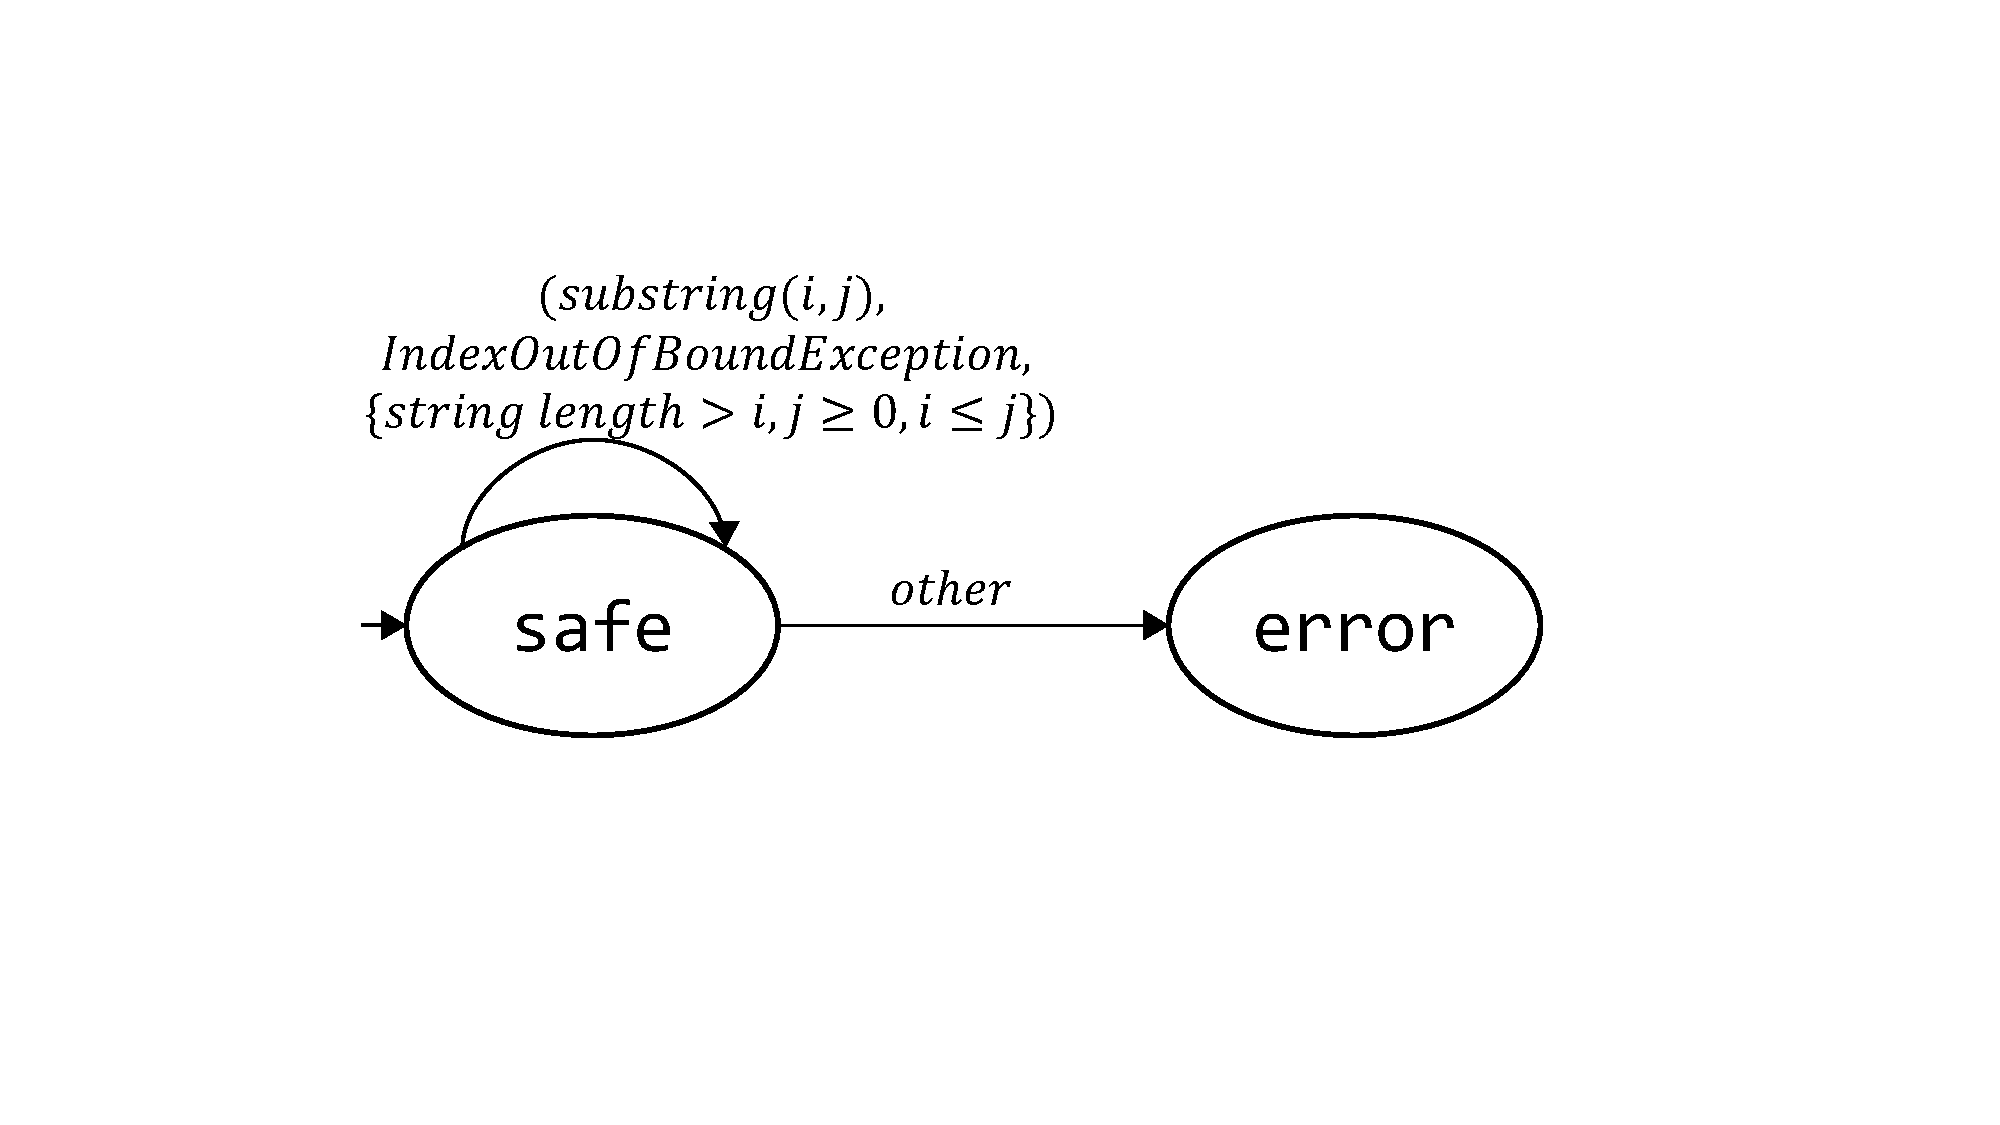
\includegraphics[scale=.4]{images/automataString.pdf}
\caption{Partial constraint representation model.}
\label{fig:constraintautomata}
\end{figure}

% An abstract constraint representation model is depicted in
% Figure~\ref{fig:constraintautomata}. A concrete model be constructed using an
% exception-specific information that is available in the API documentation. The
% repairing mechanism gets triggered when some $\eta$ is thrown while performing
% $\zeta$ after at least one of the constraints from $\Lambda$ on the structure of
% the associated string is violated. The patches essentially support the same
% semantics using multiple \code{catch} blocks corresponding to various
% exceptions.


A partial constraint representation model is depicted in
Figure~\ref{fig:constraintautomata}. It essentially specifies the constraints
that are associated with \code{substring}
method and \code{IndexOutofBoundException} exception that can be thrown by the
method. A complete model would
have several such self-looping transitions corresponding to other \java\
\code{String} API methods. The
repairing mechanism gets triggered when an exception is thrown while performing
a string operation after at least one of the constraints on the structure of
the associated string is violated. This is represented by the transition labeled
by \code{other}. The patches essentially support the same
semantics identified by the transitions with the help of \code{catch} blocks.

%------------------------

\section{Limitations}
\label{sec:tool:limitation}

\tool's major limitation arises from the fact that it is heavily directed
towards repairing handling \code{String} objects and API exceptions. While this
may seem to be a limitation, we believe that \tool's strength lies in the fact
that it mines contextual data about runtime exceptions related to \code{String}
objects that helps development of intelligent program patches. Moreover, \tool's
technique is generic and can be ported to any other class of \java\ APIs.

\tool generates precise patches considering the program context which avoids
cascading exceptions to a great extent producing the intended behavior in case
of failures. However, it still cannot give guarantees about elimination of cascading
exceptions, particularly when there are heavy object dependencies in the program.

The quality of \tool's patches also depends on the nature of the constraint
solver, which is pluggable. A more sophisticated solver may improve the quality
of program repair, and we leave comparison of different solvers for future work.

\ignore{
\paragraph{Identifying Program Statements.} We perform static taint analysis
to identify sensitive data which are leaving the system via database, network
stream, file stream or console. Providing patches to the
statements that manipulate this data would be undesirable, since
activation of the patches in case failures may allow altered sensitive data to
eventually
reach users. Hence, we only mark those program statements which do
not manipulate these data.

\paragraph{Noninvasive Patching.} In case a runtime exception that is thrown
by a statement as a result of a failure is already caught and handled in a
program,
we skip that statement from patching to avoid interfering with the results. Such
statements are identified by analyzing call-graphs and ensuring that no caller
method
in the call-chain handles the exception or its superclass. By embedding the
patches inside
\texttt{catch} blocks, we ensure that they do not get activated during normal
program execution.

\paragraph{Patch Generation.} We first perform an
intra-procedural static analysis
to identify constraints on the string objects under consideration. By
identifying
the type of exceptions that can be thrown in case of a failure, we
develop patches that
regenerate string objects by tweaking \java\ \code{String} API used in
the statements to regenerate legal string objects and by trying to solve the
constraints. In the latter case,
we evaluate the constraints statically if complete information is available at
the compilation-time. Otherwise, the analysis automatically generates
code that performs dynamic analysis to solve the constraints, and then
inserts this code in the generated patches.

\paragraph{Optimizing Instrumentation.} We perform reaching definitions
analysis to skip marked statements
if the string variables that are contained in the statements are already
patched, and the variables
are not redefined along any path that originates from the patched statement.
This analysis reduces
instrumentation points in a program.

\paragraph{Patch Precision.} The precision of a program patch is improved,
firstly, by targeting only strings
for patching which allows us to develop more specialized patches, secondly, by
patching programs very
close to the points of potential failures which avoids unnecessary patching of
other
unaffected variables and their potential
side effects, thirdly, by analyzing the types of exceptions that can be thrown
which
provides valuable insights into
origins of failures, and finally, by considering all the constraints
on the strings. This would result
in a program behavior closed to the intended one in case of a failure.

\paragraph{Reduced Overhead.} The side-effect of non-invasive patches is that
they do not interfere during
normal execution which results in no runtime overhead. Even when they get
activated in case of failures,
they still cause negligible overhead since we perform no analysis during runtime
except if required resolve the dynamic constraints.
As our study reveals~\xref{sec:evaluation} the constraints are typically few and
simple, making
the dynamic analysis light-weight.
}


%%%%%%%%%%%%%%%%%%%%%%%%%%%%%%%%%%%%%%%%%%%%%%%%%

%%%%%%%%%%%%%%%%%%%%%%%%%%%%%%%%%%%%%%%%%%%%%%%%%
%Implementation
\chapter{Implementation Details}
\label{chapter:iimplementation}

\section{Taint Analysis}
\label{sec:taintAnalysis}

For the taint analysis phase we have used \soot\ \infoflow\ framework. This
framework requires configuration files to fescribe source and sink methods. We
have identified couple of methods and some of them are tabulated in the
table~\ref{tab:TaintSources} and~\ref{tab:TaintSinks} respectively. We have
extended their InfoFlow class and added methods which store the statements in a
\code{HashMap} object as \code{Unit}. The taint analysis phase takes two inputs :
the jar file of the project which is to be analyzed and the \code{SootMethod} 
signature of the entry point of that project.

\section{Call Chain Look-up for Already Handled Exception}
\label{sec:callChainLookUp}

In some scenarios, the developer may put exception handling mechanism in case
there is any runtime exception. In such cases, we shouldn't do any repairing 
as it may change the correct program behavior. There can be two cases.

\begin{itemize}

\item In the current method if the statement is wrapped in try-catch block. In \soot\
the exception handling mechanism is handle by \code{Trap} class. Each \code{Trap}
object has start, end and handler unit. From a particular \code{Unit}, we saw if 
the unit belongs to any of the existing \code{Trap} and tag the \code{Unit} in
a \code{HashMap} object so that later at the repairing phase it can be exclude
from instrumentation.

\item If the exception is handled upper in the call chain, in the case we generate 
\code{CallGhaph} using the project's entry point as the entry point of that call 
graph. For a method we did reverse Breadth First search (BFS) to see from which 
methods it is invoked and also all of its ancestors in the call chain. From there
we retrieve the information if any particular call sight was wrapped in try-catch
block or not. In such case we tag the \code{Unit} in the \code{HashMap} mentioned 
before.

\end{itemize}

\section{Constraint Analysis}
\label{sec:constraint analysis}

\subsection{Static Constraint Analysis}
\label{subsec:staticConstraint}

We did static constraint analysis for all string object to make the patch as much
close as the original object. In the static phase we see all the conditional 
statements. There can be some conditional statements where the constraint can 
be statically determined. E.g \code{if(str.length() == 5}. We collects all these
information in a custom data type and update it. For simplicity, we keep only the 
information such as minimum and maximum length, set of characters which the string
may contains and set of possible prefix. With all these information, we generate 
the string object statically. The sting generation algorithm is described in
Algorithm~\ref{algo:constraint}. 

\subsection{Dynamic Constraint Analysis}
\label{subsec:dynamicConstraint}

We performed dynamic analysis in case the constraint can not be evaluated 
statically e.g. \code{if(str.contains(inputString()))}. In such cases just
before the conditional statement we instrument the bytecode with a static 
invocation which will populate the custom constraint data type and recalculate 
the string object with already existing constraints.


\section{String Repairing Phase}
\label{sec:stringReepairing}

\begin{algorithm}
\small
\DontPrintSemicolon
\KwData{String object $Str$ and index set $IS$ which contains ${i}$ or
${i,j}$.}
\KwResult{Repaired index set containin ${Ri}$ or ${Ri,Rj}$ based on input $IS$}
\Begin
{
	$Length \longleftarrow$ length of $Str$\;
	\If{$Length == 0$}
	{
		$Ri, Rj \longleftarrow 0$\;
	}
	\Else
	{
		\If{$i \textgreater j$}
		{
			$Ri \longleftarrow j - 1$;
		}
		\If{$i \textgreater Lengrh$ \bf{OR} $j \textgreater Lengrh$}
		{
			$Ri \longleftarrow Length - 1$ or $Rj \longleftarrow Length - 1$ based on
			condition\; 
		}
		\If{$i \textless 0$ \bf{OR} $j \textless 0h$}
		{
			$Ri \longleftarrow 0$ or $Rj \longleftarrow 0$ based on
			condition\; 
		}
		
		
	}	

}
\caption{String patching based on parameters passed}
\label{algo:stringPatchParametr}
\end{algorithm}
%%%%%%%%%%%%%%%%%%%%%%%%%%%%%%%%%%%%%%%%%%%%%%%%%

%%%%%%%%%%%%%%%%%%%%%%%%%%%%%%%%%%%%%%%%%%%%%%%%%
%Benchmark Results

\chapter{Evaluation}
\label{chapter:results}

\begin{table*}[t]
% \setlength{\tabcolsep}{3pt}
\centering
\begin{tabular}{|l|c|l|r|r||r|c|r|r|c|}

\hline

\multicolumn{1}{|c|}{\textbf{API}} &
\multicolumn{1}{c|}{\textbf{Bug Ref}} &
\multicolumn{1}{c|}{\textbf{Priority}} &
\multicolumn{1}{c|}{\textbf{$\mathcal{N}_{CG}$}} &
\multicolumn{1}{c||}{\textbf{$\mathcal{N}_{Unit}$}} &
\multicolumn{1}{c|}{\textbf{$PQI$}} &
\multicolumn{1}{c|}{\textbf{$FCI$}} &
\multicolumn{1}{c|}{\textbf{$\mathcal{IC}_{NO}$}} & %instrumentation with
%optimization
\multicolumn{1}{c|}{\textbf{$\mathcal{IC}_{WO}$}} & %instrumentation without
%optimization
%\multicolumn{1}{c|}{\textbf{$\mathcal{PF}_{CA}$}} & %profile for constraint
%\multicolumn{1}{c|}{\textbf{$\mathcal{PF}_{TA}$}} & %profile for taint analysis
%\multicolumn{1}{c|}{\textbf{$\mathcal{PF}_{CG}$}} & %profile for call graph
%\multicolumn{1}{c|}{\textbf{$\mathcal{PF}_{IN}$}} & %profile for
% instrumentation
\multicolumn{1}{c|}{\textbf{$\mathcal{RS}_{CE}$}}\\ % cascaded exception

\hline
%% 1.02238806
\code{Aries} & \cite{ARIES1204} & Major &$3.5K$ &$129$  & $ 1.02$ & $0$  &$42$&
$5$

%$3.1/10$ & $0.6/31$ & $12.8/146$ &$2.3/142$
& $\checkmark$ \\
%% 0.791666667
\code{Commons CLI1.x} & \cite{CLI193} & Critical & $3.2K$ & $53$  & $0.79
 $ & $0$  & $19$& $19$

%& $2.8/5$ & $0.5/30$ & $11.6/149$ & $1.9/133$
& $\checkmark$ \\
%% 0.5
\code{Commons CLI2.x} & \cite{CLI46} & Major & $3.2K$ & $21$ & $0.50
 $ & $1$  & $13$
&$2$
%& $2.8/5$ & $0.6/32$ & $12/212$ & $2/131$
& $\times$ \\
%% 0.992753623
\code{Commons Compress} & \cite{COMPRESS26} & Blocker & $4.0K$ & $134$  & $0.99
 $ & $0$& $46$& $4$
%$2.7/5$ & $0.5/30$ & $11.5/209$ & $1.8/130$
&$\checkmark$\\
%% 1.015873016
\code{Commons IO} & \cite{IO179} & Major & $3.3K$ & $125$ & $ 1.01
$ & $0$  & $76$ & $1$
%$3/11$ & $0.5/33$ & $12/209$ & $2/141$
& $\checkmark$\\
%% 0.983870968
\code{Commons Lang} & \cite{LANG457} & Major & $5.1K$ & $240$ & $0.98
 $ & $0$  & $168$&
$8$
%$3/19$ & $0.57/30$ & $16.5/209$ & $2.8/158$
& $\checkmark$ \\
%% 1
\code{Commons Math} & \cite{MATH198} & Major & $3.4K$ & $300$ & $1.00
 $ & $1$  & $36$
&$2$
%$3/20$ & $0.5/30$ & $11.9/209$ & $2.9/152$
& $\checkmark$ \\
%% 1.066666667
\code{Commons Net} & \cite{NET442} & Major & $3.3K$ & $14$ & $ 1.07
$ & $0$  & $6$ &
$1$
%$2.8/6$ & $0.5/33$ & $11.4/212$ & $1.9/132$
& $\checkmark$ \\
%% 1
\code{Commons VFS} & \cite{VFS338} & Major &$4.5K$ & $37$ & $1.00
 $ & $0$  & $20$ & $2$

%$3.7/13$ & $1.4/7$ & $46.1/151$ & $3.1/143$
& $\checkmark$ \\
%% 0.956521739
\code{Derby} & \cite{DERBY4748} & Major & $4.4K$ &$40$ & $0.96
 $ & $0$  & $47$ & $6$
%$3.3/15$ & $0.5/31$ & $19.9/208$ & $2.7/146$
& $\checkmark$ \\
% %% 0.942857143
%  \code{DUMMY 4 compilation} & \cite{DUMMY} & Major & $3.3K$ & $33$ & $0.94$ &
%  $0$ & $13$ & $2$
%  %& $2.7/8$ & $0.5/33$ & $13.5/213$ & $2.2/131$
%  & $\checkmark$ \\
% 0.519607843
\code{Eclipse AJ Weaver} & \cite{EclipseBug432874} & Major & $20.6K$ & $50$ & $
0.52 $ &$0$  & $4$ & $1$
%& $3.1/18$ & $0.6/34$ & $41.2/212$ &$1.6/142$
& $\times$ \\
%% 1.025
\code{Eclipse AJ} & \cite{EclipseBug333066} & Major & $25.0K$ &$39$ & $1.03
 $ & $0$ & $6$ & $1$
%$3.8/24$ & $0.5/34$ & $43.6/214$ & $1.6/156$
&$\checkmark$ \\
%% 0.960
\code{FlexDK 3.4} &\cite{SDK14417} & Minor & $6.3K$ & $600$ & $0.96$ & $0$ &
$207$ & $25$
%$4.8/40$ & $0.4/31$ & $12.9/209$ & $2.6/189$
& $\checkmark$ \\
%% 0.956521739
\code{Hama 0.2.0} &\cite{HAMA212}  & Critical & $3.7K$ & $35$ & $1.38$ & $0$ &
$28$ & $5$
%$2.6/5$ & $0.5/33$ & $14.4/210$ & $3.1/134$
& $\checkmark$ \\
%% 1.015873016
\code{HBase 0.92.0} &\cite{HBASE4481}  & Critical & $4.8K$ & $61$ & $ 1.01
$ & $0$ & $13$ & $2$
%$3.2/15$ & $1.4/11$ & $18.9/212$ & $3.1/144$
& $\checkmark$\\
%% 1.015873016
\code{Hive} &\cite{HIVE6986} & Trivial &$4.4K$ & $23$ & $1.01$ & $0$  & $8$ &$1$
%$3.4/12$ & $1.5/11$ & $20/121$ & $1.6/143$
& $\checkmark$ \\
%% 0.956521739
\code{HttpClient} &\cite{HTTPCLIENT150} & Major & $3.3K$ & $14$ & $1.13$ & $0$ &
$6$& $1$
%$2.8/6$ & $0.5/33$ & $12.3/212$ & $2.7/131$
& $\checkmark$ \\
%% 1.133333333
\code{jUDDI} & \cite{JUDDI292} & Major &$3.2K$ & $70$ & $ 1.13$ & $0$  & $10$
&
$2$
%$3.1/11$ & $0.5/34$ & $13.6/209$ & $2.9/138$
& $ \checkmark$ \\
%% 0.972222222
\code{Log4j} & \cite{ApacheLog4jBug} & Major & $3.2K$ & $17$ & $ 0.97$ & $0$  &
$6$ &$1$
%$2.8/4$ & $0.5/32$ & $13/212$ & $2.5/131$
& $\checkmark$ \\
%% 1
\code{MyFaces Core} & \cite{MYFACES416} & Major  & $4.5K$ & $50$ & $1.00 $ &
$0$ & $4$& $2$
%$3.8/4$ & $0.5/30$ & $17/218$ & $1.6/130$
& $\checkmark$ \\
%% 0.980769231
\code{Nutch} & \cite{NUTCH1547} & Major & $4.5K$ & $90$ & $0.98$ & $0$  & $8$&
$1$
%$3.2/15$ & $1.2/30$ & $32.9/215$ & $3.9/147$
& $\checkmark$ \\
%% 1.010989011
\code{Ofbiz} & \cite{OFBIZ4237} & Minor & $4.4K$ & $28$ & $1.01 $ & $1$ & $6$
&$1$
%$3.1/15$ & $1.3/14$ & $18.9/215$ & $2.8/149$
& $\checkmark$ \\
%% 1.137931034
\code{PDFBox} & \cite{PDFBOX467} & Major &$4.4K$ & $23$ & $ 1.14$ & $0$  & $8$&
$1$
%$3.3/12$ & $1.5/1$ & $20/212$ & $2.6/143$
& $\checkmark$ \\
%\code{Servicemix-soap} & \cite{SMXCOMP156} & Major & High & $0$ & $$ & $$&
%$$ & $$ & $$ & $$ & $$ & $$ & $\checkmark$ \\
%% 1
\code{Sling Eclipse IDE} & \cite{SLING3095} & Major & $4.5K$ & $58$ & $ 1.00
$ & $0$ &$39$ & $6$
%$3/14$ & $0.5/34$ & $21.3/208$ & $3.5/147$
& $\checkmark$\\
%% 0.96875
\code{SOAP} & \cite{SOAP130} & Major &$5.0K$ & $165$ & $0.97$ & $1$  & $32$ &
$5$
%$3.4/19$ & $0.6/30$ & $14/209$ & $2.3/148$
& $\checkmark$ \\
%% 0.976470588
\code{SOLR 1.2} & \cite{SOLR331} & Major & $11.0K$ & $200$& $0.98$ & $0$  & $25$
& $4$
%$4.4/21$ & $0.6/32$ & $24/219$ & $2.7/139$
& $\checkmark$ \\
%% 1.024509804
\code{Struts2} & \cite{WW650} & Major &$16.0K$ & $80$ & $1.03$ & $0$  & $25$ &
$2$
%$3/14$ & $0.5/32$ & $25.9/210$ & $1.3/140$
& $\checkmark$ \\
%% 0.975609756
\code{Tapestry 5} & \cite{TAP51770} & Major & $6.2K$  & $71$ & $0.98 $ & $0$ &
$31$ &$5$
%$2.9/10$ & $0.5/34$ & $2.4/211$ & $1.9/136$
& $\checkmark$ \\
%% 0.960526316
\code{Wicket} & \cite{WICKET4387} & Major & $70.0K$ & $68$ & $0.96$ & $0$  &
$16$ & $1$
%$3/14$ & $0.5/32$ & $52.4/210$ & $1.4/142$
& $\checkmark$ \\
%% 1.028985507
\code{XalanJ2} & \cite{XALANJ836} & Major & $3.3K$ & $33$ & $ 1.03$ & $0$  &$13$
& $2$
%$2.7/8$ & $0.5/33$ & $13.5/213$ & $2.2/131$
& $\checkmark$ \\

\hline

\end{tabular}

\caption*{

\centering
\setlength{\tabcolsep}{3pt}
\begin{tabular}{ll|ll}

$\mathcal{N}_{CG}$ & \# nodes in call graph & 
$PQI$ & Patch Quality Index \\

$\mathcal{IC}_{NO}$ & Instrumentation w/o optimization
(recall \xref{sec:optimizations}) &
$\mathcal{N}_{Unit}$ & \# \code{Units} analyzed \\

$FCI$ & Flow Consistency Index &
$\mathcal{IC}_{WO}$ & Instrumentation w/ optimization (recall
\xref{sec:optimizations}) \\

$\mathcal{RS}_{CE}$ & Cascaded exception exists \\

\end{tabular}
}


\caption{\tool's accuracy results when applied to $30$ bugs in popular
open-source libraries.}
\label{tab:results}
\end{table*}



\begin{table*}[t]
% \setlength{\tabcolsep}{3pt}
\centering
\begin{tabular}{|l||c|c|c|c|}

\hline

\multicolumn{1}{|c||}{\textbf{API}} &
\multicolumn{1}{c|}{\bf{$\mathcal{PF}_{CA}$}} & %profile for constraint
\multicolumn{1}{c|}{\bf{$\mathcal{PF}_{TA}$}} & %profile for taint analysis
\multicolumn{1}{c|}{\bf{$\mathcal{PF}_{CG}$}} & %profile for call graph
\multicolumn{1}{c|}{\bf{$\mathcal{PF}_{IN}$}} \\

\hline

\code{Aries} & $\ \ 3.1/10\ \ $ & $\ \ 0.6/31\ \ $ & $\ \ 12.8/146\ \ $ &
$\ \ 2.3/142\ \ $\\
\hline
\code{Commons CLI1.x}& $2.8/5$ & $0.5/30$ & $11.6/149$ & $1.9/133$\\
\hline
\code{Commons CLI2.x} & $2.8/5$ & $0.6/32$ & $12/212$ & $2/131$ \\
\hline
\code{Commons Compress} & $2.7/5$ & $0.5/30$ & $11.5/209$ & $1.8/130$\\
\hline
\code{Commons IO} & $3/11$ & $0.5/33$ & $12/209$ & $2/141$\\
\hline
\code{Commons Lang} & $3/19$ & $0.57/30$ & $16.5/209$ & $2.8/158$\\
\hline
\code{Commons Math} & $3/20$ & $0.5/30$ & $11.9/209$ & $2.9/152$\\
\hline
\code{Commons Net} & $2.8/6$ & $0.5/33$ & $11.4/212$ & $1.9/132$\\
\hline
\code{Commons VFS} & $3.7/13$ & $1.4/7$ & $46.1/151$ & $3.1/143$\\
\hline
\code{Derby} & $3.3/15$ & $0.5/31$ & $19.9/208$ & $2.7/146$\\
\hline
\code{Eclipse AJ Weaver} & $3.1/18$ & $0.6/34$ & $41.2/212$ &$1.6/142$\\
\hline
\code{Eclipse AJ} & $3.8/24$ & $0.5/34$ & $43.6/214$ & $1.6/156$\\
\hline
\code{FlexDK 3.4} & $4.8/40$ & $0.4/31$ & $12.9/209$ & $2.6/189$\\
\hline
\code{Hama 0.2.0} & $2.6/5$ & $0.5/33$ & $14.4/210$ & $3.1/134$\\
\hline
\code{HBase 0.92.0} & $3.2/15$ & $1.4/11$ & $18.9/212$ & $3.1/144$\\
\hline
\code{Hive} & $3.4/12$ & $1.5/11$ & $20/121$ & $1.6/143$ \\
\hline
\code{HttpClient} & $2.8/6$ & $0.5/33$ & $12.3/212$ & $2.7/131$\\
\hline
\code{jUDDI} & $3.1/11$ & $0.5/34$ & $13.6/209$ & $2.9/138$\\
\hline
\code{Log4j} & $2.8/4$ & $0.5/32$ & $13/212$ & $2.5/131$\\
\hline
\code{MyFaces Core} & $3.8/4$ & $0.5/30$ & $17/218$ & $1.6/130$\\
\hline
\code{Nutch} & $3.2/15$ & $1.2/30$ & $32.9/215$ & $3.9/147$\\
\hline
\code{Ofbiz} & $3.1/15$ & $1.3/14$ & $18.9/215$ & $2.8/149$\\
\hline
\code{PDFBox} & $3.3/12$ & $1.5/1$ & $20/212$ & $2.6/143$\\
\hline
\code{Sling Eclipse IDE} & $3/14$ & $0.5/34$ & $21.3/208$ & $3.5/147$\\
\hline
\code{SOAP} & $3.4/19$ & $0.6/30$ & $14/209$ & $2.3/148$\\
\hline
\code{SOLR 1.2} & $4.4/21$ & $0.6/32$ & $24/219$ & $2.7/139$\\
\hline
\code{Struts2} & $3/14$ & $0.5/32$ & $25.9/210$ & $1.3/140$\\
\hline
\code{Tapestry 5} & $2.9/10$ & $0.5/34$ & $2.4/211$ & $1.9/136$\\
\hline
\code{Wicket} & $3/14$ & $0.5/32$ & $52.4/210$ & $1.4/142$\\
\hline
\code{XalanJ2} & $2.7/8$ & $0.5/33$ & $13.5/213$ & $2.2/131$\\
\hline

\end{tabular}

\caption*{
\centering
\setlength{\tabcolsep}{3pt}
\begin{tabular}{ll|ll}

$\mathcal{PF}_{CA}$ & Profiling for constraint analysis phase &
$\mathcal{PF}_{TA}$ & Profiling for taint analysis phase \\

$\mathcal{PF}_{CG}$ & Profiling for call graph phase &
$\mathcal{PF}_{IN}$ & Profiling for instrumentation phase \\


\end{tabular}
}


\caption{\tool's profiling results for time and memory footprint}
\label{tab:profile}
\end{table*}



We now present an evaluation of \tool. In \xref{sub:accuracy}, we evaluate
\tool's effectiveness by measuring the quality of patches and related
instrumentation required. We also measure how the several optimizations
described in \xref{sec:optimizations} affect the patches generated by \tool.
In \xref{sub:overhead}, we measure the relative performance and resource
penalties incurred with \tool. In \xref{sub:casestudies}, we describe our
experiences with some of the major bugs from our data set.

\myparagraph{Data Set} We mined bug repositories of several open-source
\java-based applications and selected $30$ bugs, majority of them being rated
either major, critical or blocking. These bugs involved usage of $64+$ different
APIs from \java's \code{String}, \code{StringBuffer}, \code{StringBuilder}, and
Apache \code{StringUtils} and Google Guava \code{StringUtils} classes.

% \begin{mylist}
% 
% \item \textbf{Popularity}: How much it is used among the developers and
% industries,
% \item \textbf{Severity} : We consider major, critical and blocker priority bugs
% only considering the facts at the bug affects dependent applications and other
% libraries severely.
% \item \textbf{Age and state} : We consider latest bugs which were reported in
% the last 5 years.
% We also consider such bugs which still remains un-fixed.
% 
% \end{mylist}

\myparagraph{Experimental Setup} All our experiments were performed on a laptop
with $2.9$ GHz dual core Intel i$5$ CPU, and $8$ GB of RAM, and running
Microsoft Windows $8.1$. We used JDK v$1.7$ running with $2$ GB of allocated
heap space. All bug reproduction was done on Eclipse Juno IDE. We used \soot\
v$2.5.0$ for bytecode analysis and instrumentation, and \infoflow\ snapshot
from May'14 for static taint analysis.
% We have also used \java\ decompiler JD v0.7.

% 
% equipped with a dual core Intel i5
% 2.3-2.9 GHz processor, 8 GB or RAM, Microsoft Windows 8.1 operating system, JDK
% version 1.7-45 with 2 GB of allocated heap space. All the bug reproduction was
% done on
% Eclipse Juno IDE. For static analysis and instrumentation we have used \soot\
% version 2.5.0 and \soot\ \infoflow\ for static taint analysis. We have also used
% java decompiler JD version 0.7.0.1. 

\section{Accuracy}
\label{sub:accuracy}

We evaluate the precision of the patch and the effectiveness of \tool\ based on
several metrics as described below.

% We have conducted the evaluation based on the matrices which empirically
% measures the precision and the performance of the developed tool. We measures
% the precession in terms of the quality of the patch and some other criteria
% listed bellow and the performance based on the time taken and the memory
% footprint.

\begin{itemize}

\item \textbf{Effectiveness of the patch}: Precision and effectiveness of a
patch is governed by the similarity between a \tool\ generated patch and the
developer's fix for the same bug. We define \textbf{Patch Quality Index (PQI)}
as a measure of the effectiveness of the patch.
$$PQI = \frac{\#~Constraints_{Similar}}{\#~Constraints_{Developer}} *
\frac{\#~LOC_{Developer}}{\#~LOC_{\tool}} *
\frac{Output_{\tool}}{Output_{Developer}}$$

Specifically, PQI compares the similarities in constraints and source line of
code in \tool's patch against the developer's version, as well as the actual
output generated from both the patches, thereby considering both the logic and
the technique to construct an effective patch. A higher value of PQI is
preferred. Thus, if \tool's patch has fewer constraints, or has more lines of
code, or has fewer similarities in the output, the PQI will be lesser. 

% is the This matrix is for
% the qualitative analysis of our auto generated patches. By this measurement we
% have not only ensure the effectiveness of the patch but also look at the
% similarity of logic an patch construction with the developers' one.After the
% patching we compared both the auto-generated patch code with the developer's
% patching code we found in the bug repositories. In the case the bug is still
% un-fixed we looked for the comments and discussion in the panel and collects
% the information about the potential patch. At the first step, we visually
% compared the patches to see how much they are similar and dissimilar with the
% developers' patch.

Determining PQI is a three step process. First, we visually compared \tool's
patch with the developer's version and count the exact similar constraints
observed in both patches to determine the closeness in terms of the set of
constraints. Second, we disassembled the developer's patch and compared the
count of bytecodes generated using \tool's patch. Third, we observed the actual
output of using the \tool\ patched class files against the developer provided
patch in a later version of the same library. In case the output is primitive or
strings, an exact match is considered successful, else we iterate over the
properties of the complex object to determine number of exact matches in the two
outputs. In case of exception(s), we select the similarity ratio to be $0.5$.

% In case the results were either primitive or string type, we
% compared the output. In case the output is some complex object we compare
% the properties of them.

% Apart
% from the test cases to reproduce the bug, we also ran couple of good test case
% to make sure that the patch is not behaving any other way. Based on this
% experiment we made a metric named \textbf{Patch Quality Index (PQI)} which
% can contains three values, high, medium and low where we consider high PSI being
% a good close quality patch.


%% subsumed in PQI

% \item \textbf{Auto-generated patch size and the develops' patch size} : Apart
% from the qualitative analysis we have measured quantitative aspect of the
% Auto-generated patches and compared their sizes with the developers' one.
% Quantitative measurement comes to picture only when we are satisfied with the
% qualitative measurement. We came up with a metric called \textbf{Patch Size
% Index (PSI)}. In case our patch is qualitatively satisfactory and the size is
% less than the developer one the we assign PSI as high. In case the size varies
% in $\pm5\%$ we assign PSI as medium. If our patch is more than $5\%$ bigger than
% the develops' one then PSI is assigned to low.

Table~\ref{tab:results} lists $30$ real-world bugs mined from bug repositories
of popular open-source libraries. We wrote a driver program to recreate the bug,
and then applied \tool\ to patch it. We observed that in all cases, \tool\
successfully patched the offending class file in the concerned library.

\begin{mybullet}

 \item  We observed that PQI for \tool\ generated patches was high for most of
the bugs, which indicates the effectiveness of the patches. Specifically, for
$23$ out of $30$, \ie\ for more than $75\%$ cases, PQI for \tool-generated
patches was within $7\%$ of the developer's fix. Note that there was one
instance where the concerned bug~\cite{HBASE4481} was still unpatched. In such
cases, we looked for the potential or suggested patches in comments and
discussion forums, and compared \tool's patch with them.

 \item We observed that PQI for bug in Hama $0.2.0$~\cite{HAMA212} was as high
as $1.38$. We visually inspected both the \tool-generated patch and the
developer's fix and observed that \tool's patch was considerably smaller.
Further, we noticed that the developer's patch had i) multiple assertion blocks
to make sure the error condition can be avoided, and ii) several additional
conditional checks to avoid corner cases. Moreover, the developer's patch also
had a completely different implementation of the method on which the bug was
reported. Thus, the developer's fix was significantly larger than \tool's patch.

 \item We noticed low PQI (between $0.5$ and $0.79$) for four of the patched
libraries, which shows that the quality of the \tool-generated patch was
significantly lower than the developer's fix. A major reason for this drop in
PQI is the presence of cascaded exceptions observed in the patched versions of
these libraries upon execution.
% Though the
% repairing technique able to patch the buggy string api usage, but the patched
% version of the string was later used to load some configuration of used as a
% driver string to some place else.
We note that \tool\ in its present shape does not guarantee that the patch will
never raise cascaded exceptions. Thus, in these four cases \tool's patches were
of lower quality then the original ones. However, we also note that all the
cascaded exceptions were in fact checked exceptions, and it is expected that the
application developers would handle them appropriately.

 \item Note that taint analysis only works when sources and sinks are defined.
Since our library benchmarks have no notion of sources or sinks, \tool's
bytecode analysis of the libraries did not involve the taint analysis phase.
However, even without taint analysis, \tool's patches were of high quality, as
demonstrated by the high PQI.

\end{mybullet}

\begin{table}[t]
\centering
\begin{tabular}{|l|r|r|r|}
\hline
\multicolumn{1}{|c|}{\textbf{Application}} &
\multicolumn{1}{c|}{\textbf{KLOC}} &
\multicolumn{1}{c|}{\textbf{Total paths}} &
\multicolumn{1}{c|}{\textbf{Tainted paths}}\\

\hline
\code{Checkstyle}& $58.0K$ & $1977$ & $88$\\
\code{Jazzy Core}& $4.9K$ & $270$ & $26$\\
\code{JEdit}& $4.3K$ & $185$ & $22$\\

\hline
\end{tabular}

\caption{Precision results for taint analysis.}
\label{tab:taintAnalysis}
\end{table}

\item \textbf{Precision of taint analysis}: \tool\ leverages off-the-shelf
tools (\infoflow) to perform the taint analysis. We measure precision of our
choice of tool by measuring the number of statements in the analyzed code that
are deemed unsafe to patch. Since we could not measure the precision of our
taint analysis on the library benchmarks (as discussed earlier), we select $3$
diverse applications and apply \tool\ in its entirety to obtain a measure of the
precision of the taint analysis. Specifically, for each application we provided
a set of sources, sinks and taint propagators to \infoflow, which listed the
total number of tainted paths, \ie\ paths from a sensitive source to a sink and
thus must not be patched. Table~\ref{tab:taintAnalysis} lists the results. We
observe that the total number of tainted paths is less than $12\%$ across the
applications.

\myparagraph{Threats to validity} Note that \tool\ is dependent on \infoflow\
for achieving precision about the points of instrumentation. However,
\infoflow\ currently has a major limitation---it does not support taint
analysis for multi-threaded programs. Moreover, since it is still under active
development, we observed that when applied to certain applications, \infoflow\
consumed inordinate amounts of memory and crashed. Thus, \tool's precision is
limited by the accuracy of its dependencies. 

\item \textbf{Already handled exceptions}: \tool\ analyzes the call graph to
determine if a potential runtime exception throwing statement is handled higher
up in the call chain or in the same method. In such cases \tool\ must abort the
patching effort considering that the exception is caught with exact exception
type or its base type. This is required else patching will disrupt the normal
control flow of the program.

We measure the extent of this optimization, which prevents disruption of the
control flow using the \textbf{Flow Consistency Index (FCI)} that is calculated
as $$FCI = n$$, where $n$ is the number of exceptions in the application that
must be ignored \tool\ for forced patching of the bug. Note that $FCI \ge 0$,
and a lower value of $FCI$ is desirable. We observe that patching four bugs
required \tool\ to ignore at most one exception; rest required no changes.

\item \textbf{Cascaded exceptions}: A cascaded exception arises if the
\tool-generated patch creates objects that when used as inputs to other \java\
APIs result in further exceptions.
% patched objects
% are used as a input
% to other methods and violates the specification there.
\tool\ is prone to cascading exceptions because of the limitation of its
intra-procedural analysis and a simple constraint evaluation mechanism. However,
\tool's constraint solver is pluggable and a more sophisticated third party
solvers can easily be integrated.
% This is the limitation
% in our technique in the some complicated cases where it requires develops' 
% attention. The limitation is due to the fact that the analysis for the
% repairing 
% technique is a intra-procedural analysis and the constraint evaluation method is
% very simple. For the constraint evaluation part, the solver is pluggable, we can
% easily replace it with a third party solver.
Specifically, cascaded exceptions may arise if the patch generates \code{String}
objects that represent a malformed string. Further, if we keep the optimization
in \xref{subsec:minimizePatchInstrumentation}, then cascaded failures may
occur even for subsequent \code{String} APIs handling the malformed
string following the point of patching. If the optimization is turned
off, \tool\ will automatically patch all relevant \code{String} APIs and thus
handle all cascaded failures involving malformed \code{String} objects.
% 
% Cascaded exception can be noticed
% when the string object we are patching is generation some specific URI or driver
% string which would be used to load or configure something. In such scenario, the
% patch may produce some malformed string. In case there is a cascaded exception 
% in string object, our analysis will take care of it, other wise it would
% abort.

We observe that two benchmarks throw cascaded exceptions even after being
repaired. The cascading was one level deep and triggered exception in another
non-String code (and thus unpatched), which caused the application to crash.

\end{itemize}

Detailed evaluation for each of the bugs in our data set is available at
\url{http://goo.gl/d1zcXD}.

\section{Overhead}
\label{sub:overhead}

We measure the overhead of \tool\ across different metrics identified below.

\begin{figure*}[t]
\centering
\begin{tabular}{ccc}
\subfloat[Variation in call graph analysis time with size of call
graph.\label{fig:perf:callgraph}]
{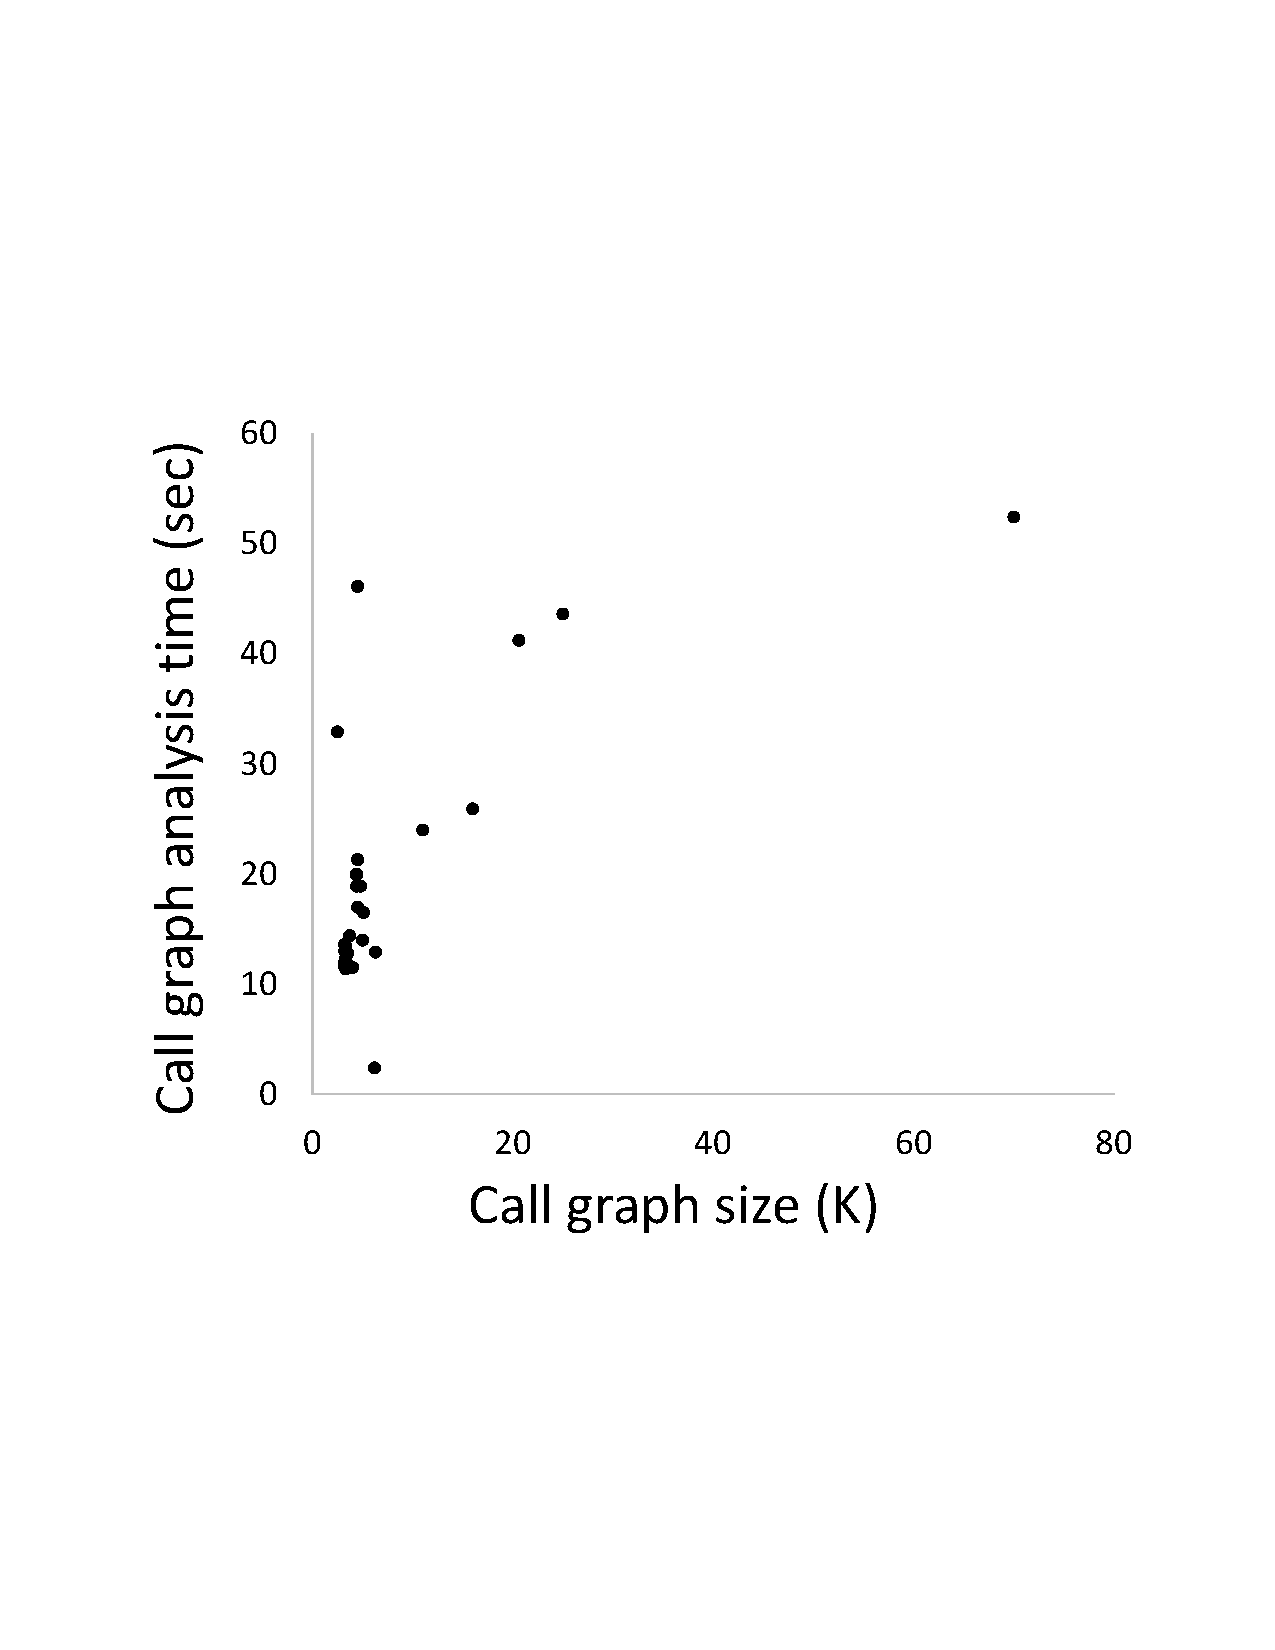
\includegraphics[width=.3\linewidth]{images/CgSizeVsTime.pdf}}
\hfill
&
\subfloat[Variation in static constraint analysis time with number of
constraints.\label{fig:perf:constraints}]
{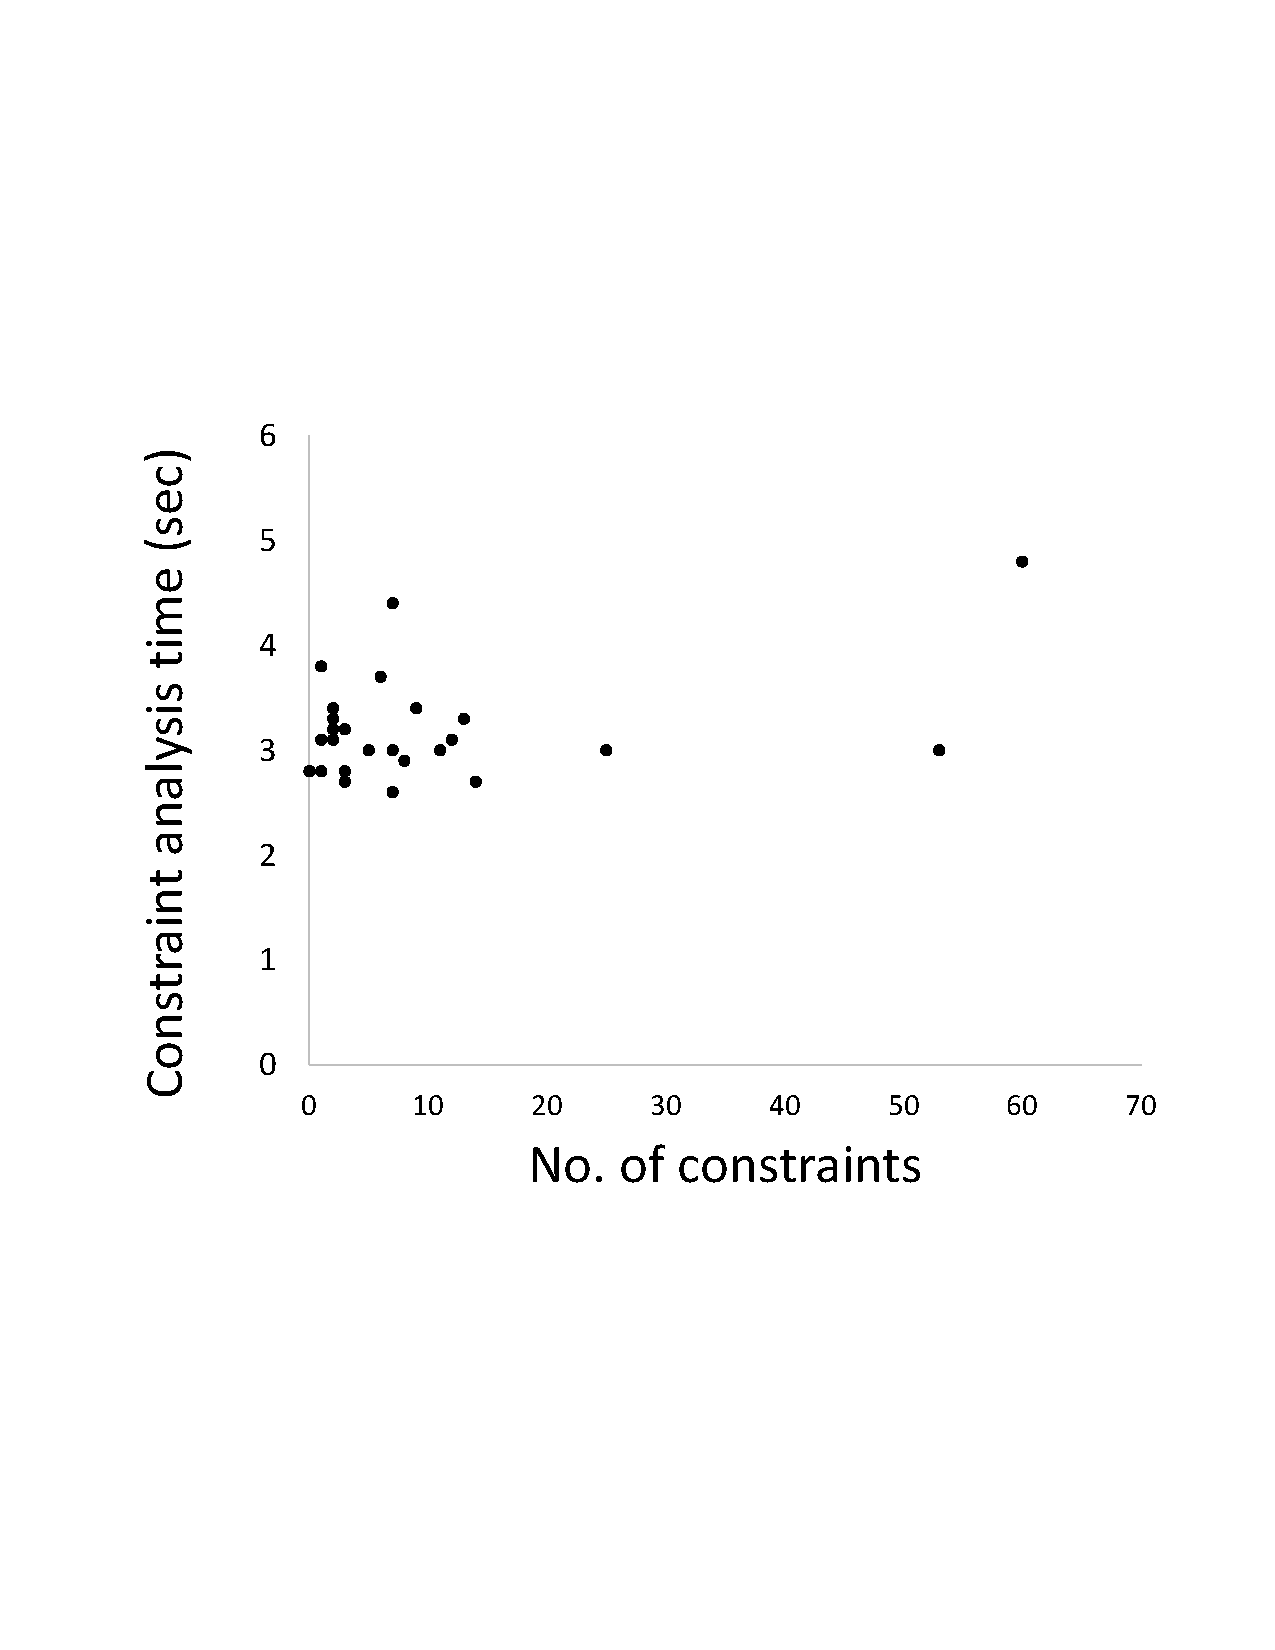
\includegraphics[width=.3\linewidth]{images/ConstraintsVsTime.pdf}
}
\hfill
&
\subfloat[Variation in instrumentation time with \code{Units} to be
instrumented.\label{fig:perf:units}]
{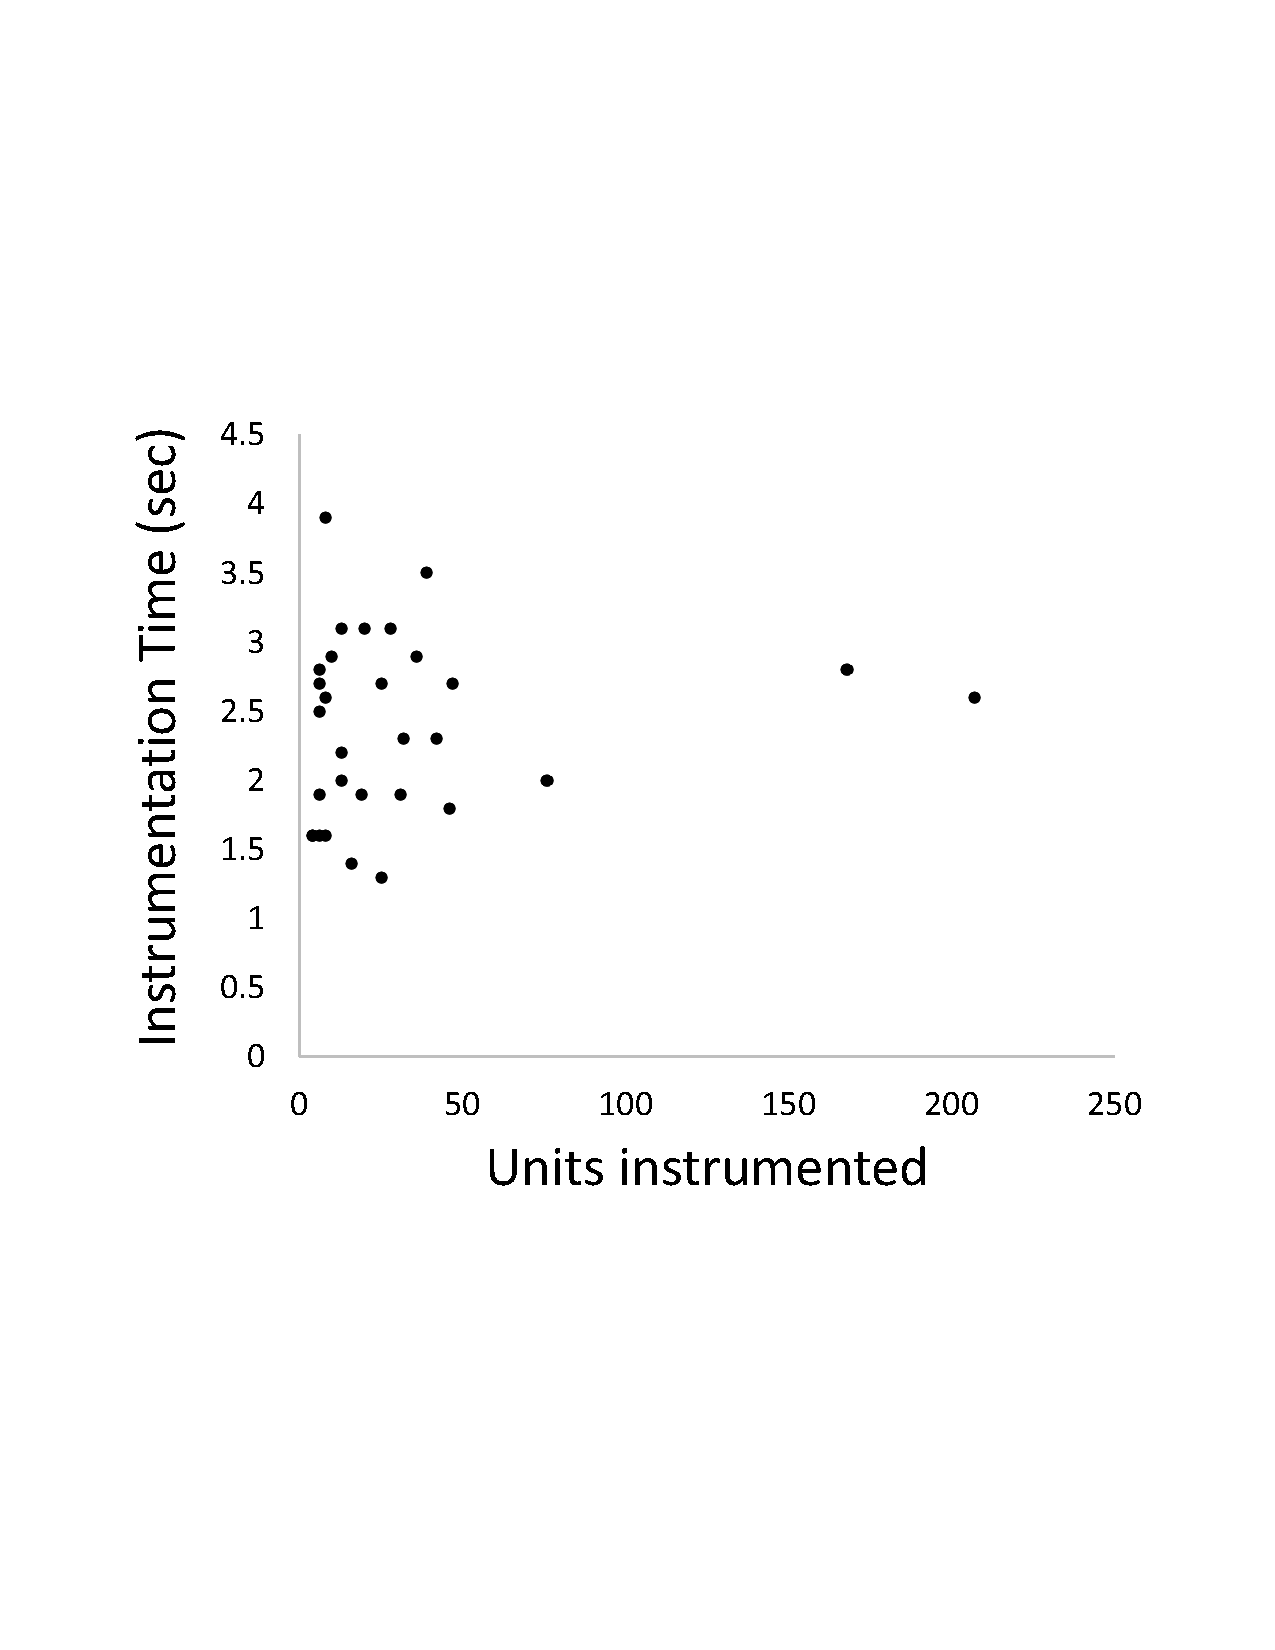
\includegraphics[width=.3\linewidth]{images/InstrumentationVsTime.pdf}}
\hfill
\\
\end{tabular}
\caption{\tool\ evaluation.}
\end{figure*}

\begin{itemize}

% Apache wicket 100K run patched -> 1090ms, dev fix -> 929 ms
% Eclipse AspectJ weaver 50K run patched -> 8ms, dev fix -> 2 ms
% Apache Tapestry 50K run patched -> 200ms, dev fix -> 178 ms
% Nutch -> 50k run, patched ->183ms, dev patched-> 12 ms
% Hive -> 50k run, patched ->297ms, dev patched-> 99ms

% Constraint analysis dependency : soot invoke + it flashes jimple files.
% 
% Instrumentation dependency : soot overhead for instrumentation  + flashes
% instrumented class files to disk.
% 
% call graph dependency : apart from soot none

 \item \textbf{Execution overhead}: We randomly selected and patched $5$
libraries (Apache Tapestry, Apache Wicket, Eclipse AspectJ Weaver, Hive and
Nutch) from Table~\ref{tab:results} to determine the execution overhead of the
patched class files. We observed that \tool\ reports an average overhead of
$\sim$$2.32\mu$s per call across the $5$ benchmarks for $50K$ runs of the
patched functionality in both the developer's version and \tool's patched
library. The maximum absolute overhead was observed for Hive at $\sim$$3.96\mu$s
per call. The above overhead is imperceptible at human response time scales.

 \item \textbf{Call graph}: The size of the call graph directly governs the time
and memory consumption for \tool. Figure~\ref{fig:perf:callgraph} shows the
results for the benchmarks analyzed from our data set. The overall analysis
time was under a minute for all the benchmarks. We observed that even for a call
graph of $\sim$$70K$ nodes (for \code{Wicket}), \tool\ required just $52.4$s
and $210$MB memory.

 \item \textbf{Constraint set}: \tool\ performs an exhaustive multi-pass
analysis to gather and evaluate the set of constraints for generating patches. A
higher number of constraints and their complexity increases the duration of
\tool's analysis. Figure~\ref{fig:perf:constraints} compares the time required
for static constraint collection and evaluation with an increasing number of
constraints for the benchmarks used in our data set. We observe that across
all the benchmarks used, \tool\ required at most $\sim$$5$s for collecting and
evaluating the constraints.

\item \textbf{Instrumentation overhead}: \tool\ performs bytecode
instrumentation for actual patching. Figure~\ref{fig:perf:units} shows the
variation in instrumentation time with increasing number of \code{Units} to be
patched. We observe that even without optimization discussed in
\xref{sec:optimizations}, \tool\ takes under $4$s to instrument all
\code{Units} across all benchmarks. We believe that this time would be even
less with the optimizations enabled, which significantly decrease the number of
\code{Units} to be instrumented, and is evident in Table~\ref{tab:results} where
column $\mathcal{IC}_{WO}$ is much less than $\mathcal{IC}_{NO}$.

%  \item \textbf{Number of \code{String} objects}: \tool\ performs exhaustive
% optimizations to limit the static and dynamic instrumentations at points of
% interest. Thus, \tool's performance is also dependent on the number of
% \code{String} objects. Figure~\ref{fig:perf:strings} plots the trend in analysis
% time as a function of the \code{String} objects generated for our benchmarks.
% We observer that \todo{Add details later.}.

\end{itemize}

\section{Case studies}
\label{sub:casestudies}

We now report on experiences gained when using \tool\ to patch several of the
bugs reported in Table~\ref{tab:results}.

\begin{itemize}

 \item The bug~\cite{ARIES1204} as reported in the repository for Apache Aries
cited String related issues. However, our investigation showed that the bug was
actually in the ASM framework that was invoked by Aries, and not in the was
actually not in the Aries framework as originally reported. Thus, we patched the
particular ASM methods containing the bugs, and retested it with the Aries
framework to ensure conformance.

 \item The bug in Commons Math~\cite{MATH198} had a bug related to incorrect
formatting of the input string. However, it threw a completely irrelevant
exception (\code{IndexOutOfBound}) instead of the \code{NumberFormatException},
which contains the information of the malformed string. The \tool-generated
patch fixes the undesirable behavior.

 \item The bug in OfBiz~\cite{OFBIZ4237} throws a custom shutdown exception,
when in fact it should throw a \code{StringIndexOutOfBoundsException} due to a
\code{substring} invocation with incorrect bounds. This ultimately causes the
library to throw some high priority exception and ultimately crash if not handed
properly by the application. The patched version of the library catches the
correct exception.

 \item The code to trigger bugs in some libraries, including Apache Commons
Compress, Commons Lang, Commons Math and Ofbiz, each had string operations
wrapped in \code{try-catch} block that were handled by \code{Exception} class,
\ie\ the base type of all exceptions. However, \tool\ checks for already
handled runtime exceptions during its call graph analysis, and thus did not
patch the bugs. We turned off the call graph analysis module to force \tool\ to
generate the relevant patch for the bug.

 \item We also noticed several instances where the developer code does not
follow proper programming practices regarding exception handling. For example,
the SOAP bug~\cite{SOAP130} was reported for a faulty \code{substring} call that
threw a \code{StringIndexOutOfBoundsException}. The entire method was wrapped in
a \code{try-catch} that included the faulty substring call along with other
servlet operations. However, the \code{catch} block handled the generic
\code{Exception}, which is the base class of all exceptions. Thus, both servlet
exceptions or \code{IndexOutOfBoundException} from the \code{substring} call
were handled in a generic fashion. \tool's patched library ensures that
exceptions originating from the \code{substring} call are handled properly.

\end{itemize}

%%%%%%%%%%%%%%%%%%%%%%%%%%%%%%%%%%%%%%%%%%%%%%%%%

%%%%%%%%%%%%%%%%%%%%%%%%%%%%%%%%%%%%%%%%%%%%%%%%%
%Conclusion and Future Works

\chapter{Conclusion and Future}
\label{chapter:conclusionFutureWorks}
%%%%%%%%%%%%%%%%%%%%%%%%%%%%%%%%%%%%%%%%%%%%%%%%%

\onehalfspacing
%\newpage
%\bibliographystyle{these}
\bibliographystyle{acm}
%\bibliographystyle{elsart-harv}
%\newpage
%\section{References}
%\bibliography{Library}
\bibliography{Aritrabib}

\chapter*{Appendix}
\label{chapter:appendix} 

\end{document}
